% Chapter Template
\chapter{Data and simulated datasets} \label{Chapter4} 


Nearly all of the signals which can be studied at CMS are
expected to have their potential backgrounds in which standard
processes sporadically have fluctuations that make them appear more exotic than they truly are.
For example, an isolated high \pt electron can be a ``smoking gun'' for
a few rare processes. At the same time an electron contained in a b
jet is hardly ever isolated, but since the total b jet cross section
is extremely large, even a small portion can be critical. It becomes
crucial to have a sort of ``litmus test'' to cross-check the observed
outcomes with the expected features and the predicted amount of events.
The idea is to validate the observed information by comparing it to
generated events. For this reason collision events are simulated for
several physics processes as they are predicted from theory. The
detector simulation response is taken into account. \\
In a simplistic way we can summarize a number of applications of event
generators as follows: to give analyzers a sense of the type of
events to expect and at which rates; to help in planning new
experiment designs hence detector performances are optimal for the
desired physics search; to help in drafting analysis strategies which
can be applied to data but that have been optimized a priori without
any possible unconscious bias; to estimate detector calibrations and acceptance
corrections; and to have a appropriate framework inside which to
interpret the meaning of observed physics phenomena in the optics of a
fundamental underlying theory (SM).



\section{Event simulation}\label{sec:c4eventsimulation}

The event simulation is based on the Monte Carlo (MC)
method~\cite{mc}. The simulated events
 are grouped in a specific
sample for each physics process which are called MC samples.\\
The full simulation chain is divided in separate generation stages:
\begin{itemize}
\setlength\itemsep{-0.1em}
\item \textbf{Matrix element (ME) calculation.} The ME calculation
  makes use of a list of PDFs (Parton Distribution Function) for the initial state
  depiction; a MC generator is used for the computation of the
  partonic interaction.
 For the signal samples produced specifically for this thesis and for
  most SM processes here presented, the software
  \texttt{MadGraph5\_aMC@NLO}~\cite{Alwall_2014} is used. For a few other background processes it
  the \texttt{POWHEG}~\cite{Alioli_2010} software is used. Both
  softwares have LO and NLO accuracy in QCD. For proton PDFs, in both
  generators, the NNPDF3.0~\cite{Ball_2015} and
  NNPDF3.1~\cite{Ball_2017} PDFs are used as inputs.
\item \textbf{Parton shower simulation.} The simulation is done with
  the \texttt{PYTHIA 8}~\cite{Sj_strand_2008, Sj_strand_2015}
  software. The parton shower step is necessary to address some aspects
  of the collision with regards to the evolution of quarks and gluons into jets of
  hadrons, so called \emph{hadronization}. The hadronization is
  simulated starting from an energy scale of 1 GeV, adopting phenomenological models tuned to
  experimental results~\cite{Skands_2014, Khachatryan_2016_ps, Sirunyan_2020_ps}.
\item \textbf{Detector simulation.} The detector simulation is done
  with \texttt{GEANT4}~\cite{AGOSTINELLI2003250} software. The
  simulation is based on an accurate geometrical model of the CMS
  detector, hence it includes all the material budget and it tracks
  the authentic sub-detector responses. Particle interactions with
  matter are simulated and their energy deposit is reproduced according to the
  energy and the mass of the particle and the material that it goes through. Data collected by CMS are used to
  parametrize the real detector response of each single
  sub-detector. Furthermore the trigger system and the readout system
  is mimicked. 
\end{itemize}

The events in the simulated samples appear in the same format as the
one used in data-taking. Furthermore there are single year campaigns for
each year of data-taking which correspond to different detector
conditions for each period. 
 

\section{Standard Model processes}\label{sec:c4sm}
In this section an overview is given of the SM processes (refer to Figure~\ref{fig:crosssection}) which
compose the background in the multilepton final state. The focus is
specifically on three light leptons final states, which is the
signature given by HNL decaying either into \PZ or into \PW where the bosons
decay leptonically; this final state is presented in
Chapters~\ref{Chapter5} and~\ref{Chapter6}.
\begin{figure}[h]
\centering
  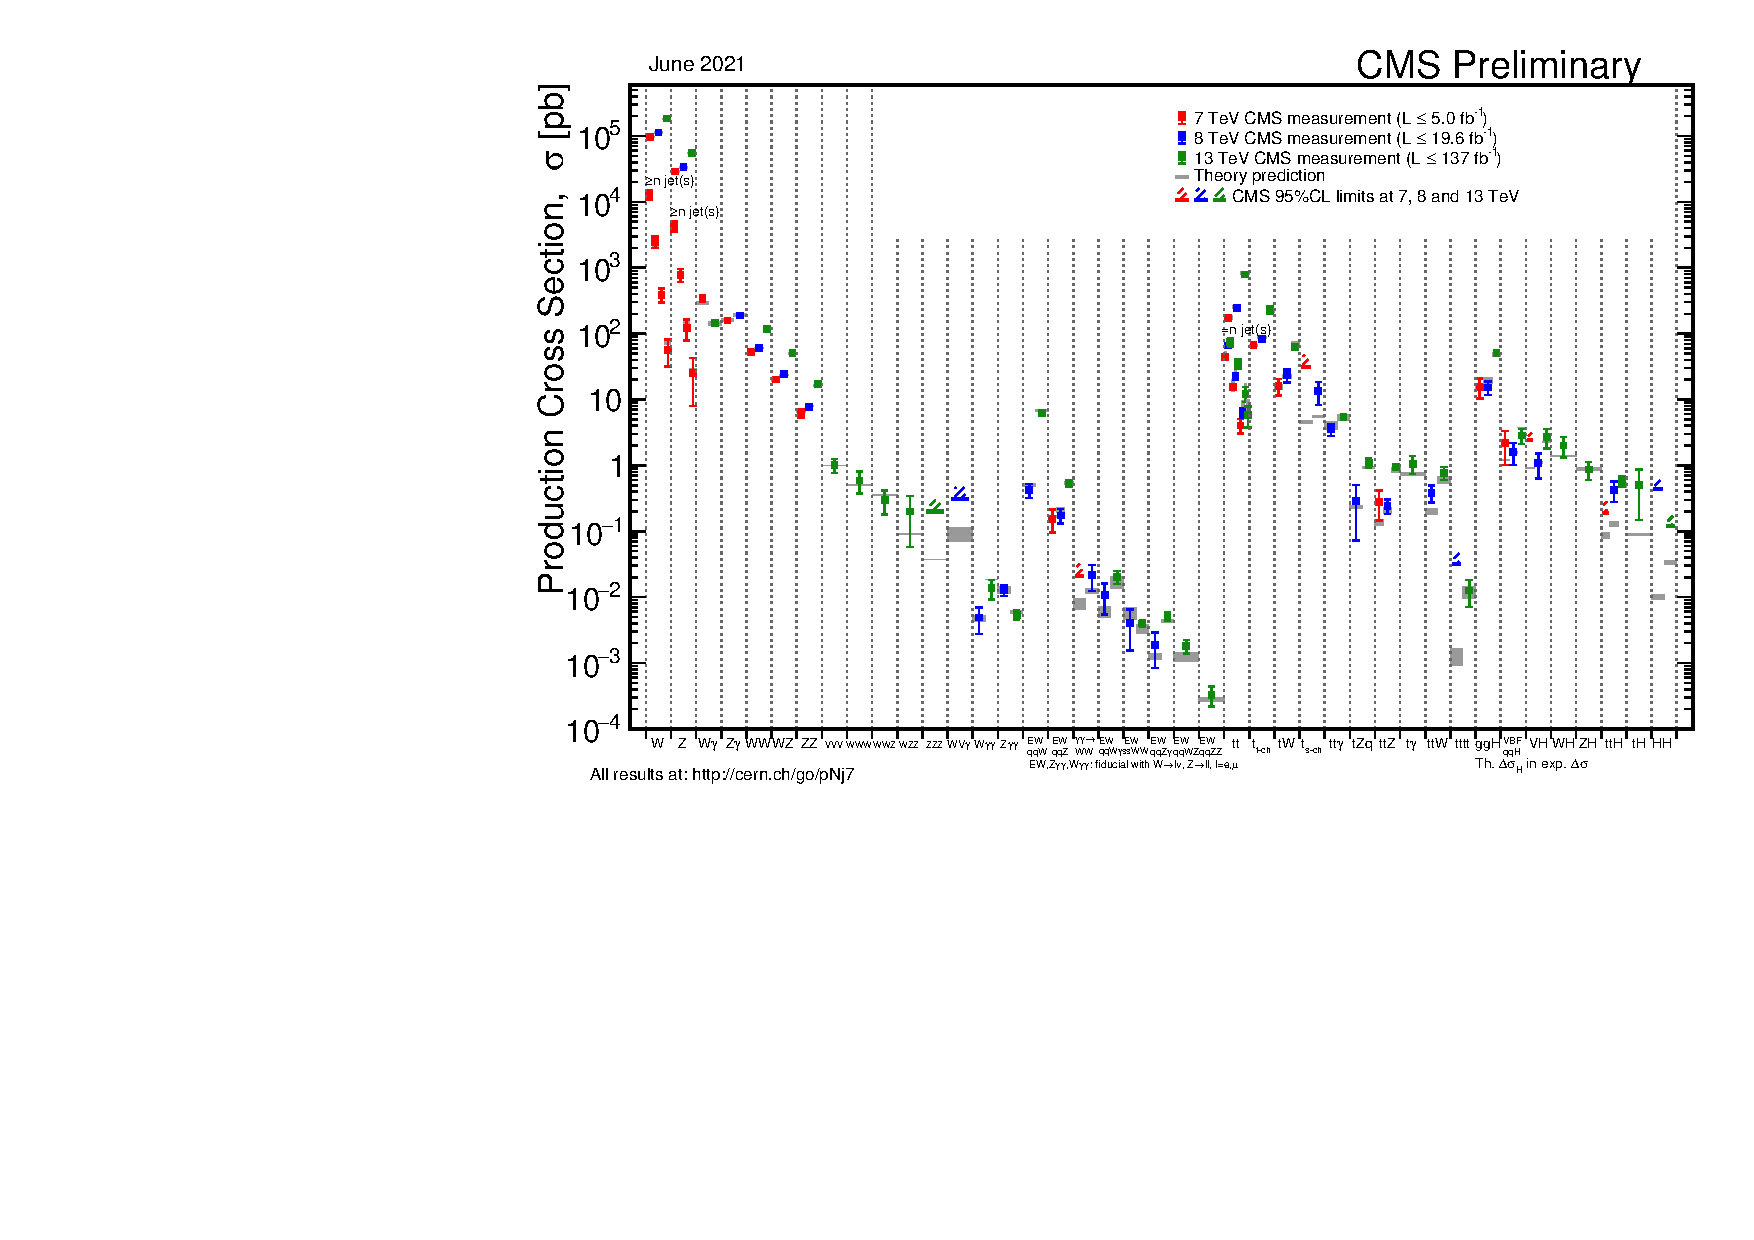
\includegraphics[width=0.95\textwidth]{Figures/c4/SigmaNew_v0.pdf}
  \caption{Summaries of cross sections measurements by CMS~\cite{cmspublic} for
    different center-of-mass energies compared to the theory
    predictions (gray). The plot gives hints about the
    amount of events we could expect from each single process and the
    relative rates with respect the signal expected yields.}
  \label{fig:crosssection}
\end{figure}

Almost all of the backgrounds are estimated from simulation using the
MC samples. The non-prompt background is the only exception and it is
discussed for each analysis separately in Sections~\ref{sec:tight_loose_method}
and~\ref{sec_llfakelepton}. 

\paragraph{Diboson production, WZ and ZZ.}\label{sec:c4wz_zz}
In case both bosons decay leptonically, the associated production of
WZ bosons produces three prompt leptons ($\PZ \rightarrow \ell^{+}
\ell^{-}$, $\PW \rightarrow \ell \nu$) and \ptmiss.
Its clear signature is an opposite sign same flavor (OSSF) pair with
invariant mass compatible with \PZ mass. The events are characterized by
having a few jets or none, and zero b jets.
WZ events
constitute a dominant background in the three prompt leptons HNL
analysis presented in Chapter~\ref{Chapter5}.

\begin{figure}[h!]
\centering
  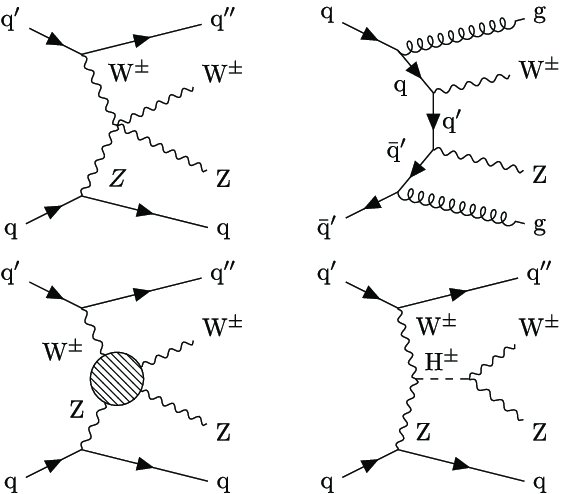
\includegraphics[height = 4cm]{Figures/c4/dia/WZjj-production.jpeg}
\hspace{1cm}
  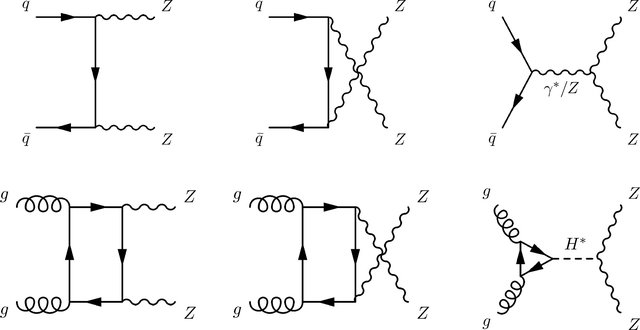
\includegraphics[height = 4cm]{Figures/c4/dia/Lowest-order-Feynman-diagrams-for-ZZ-production.jpeg}
  \caption{WZ associated production diagrams (left), ZZ associated
    production diagrams (right)~\cite{diagram}.}
  \label{fig:c41}
\end{figure}
The associated production of two \PZ bosons can enter as background in
the three lepton final states when one of the leptons fails
reconstruction or ID requirements. The events present low \ptmiss
values and they have just a few jets and zero b jets. 


\paragraph{W/Z and photon radiation.}\label{sec:c4photon}
As shown in Figure~\ref{fig:c43}, events where a boson is produced
together with a photon can extensively contribute to the background in three leptons
final states. This is the case when when a virtual photon decays (internal conversion) or in which a real photon
converts into leptons by interacting with the detector material
(external conversion). The photon undergoes an
asymmetric internal or external conversion in which one of the leptons
has very low $\pt$. This soft lepton has a high probability of failing
the selection criteria of the analysis, leading to a reconstructed
two- (in case of a $\PW$ boson) or three-lepton (in case of a $\PZ$
boson) final state. This background mostly contributes to categories
with an OSSF pair.\\
For the displaced leptons analysis presented in Chapter~\ref{Chapter6}
the external conversion is a ``nasty'' background because it can mimic
a HNL decay vertex where $e^{+}e^{-}$ is produced. In order
to reduce this background a material veto can be applied which rejects all the SV
which are located in proximity either of a detector layer or of an inert material.

\begin{figure}[h!]
\centering
  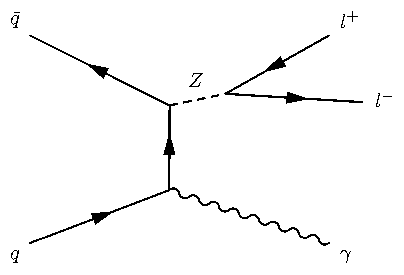
\includegraphics[width=0.2\textwidth]{Figures/c4/dia/40000101.pdf}
  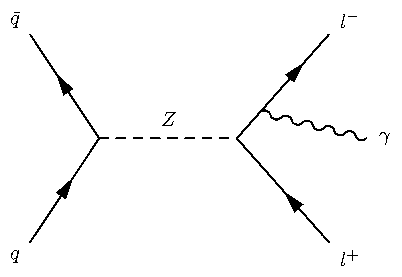
\includegraphics[width=0.2\textwidth]{Figures/c4/dia/40000104.pdf}
  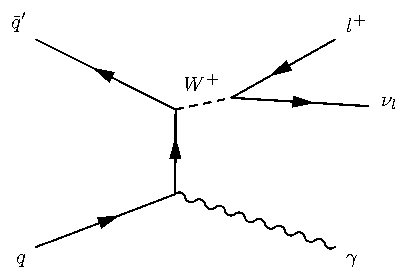
\includegraphics[width=0.2\textwidth]{Figures/c4/dia/40000111.pdf}
  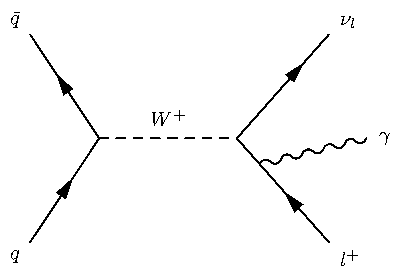
\includegraphics[width=0.2\textwidth]{Figures/c4/dia/40000114.pdf}
  \caption{\PW or \PZ plus $\gamma$ production diagrams~\cite{diagram}.}
  \label{fig:c43}
\end{figure}

\paragraph{Drell-Yan production.}\label{sec:c4dy}
The Drell-Yan process happens when a quark from one of the initial
protons annihilates with an anti-quark from a proton traveling in the
opposite direction. The quarks are converted into a $\gamma^{*}$ or
\PZ, which decays into two leptons.

\begin{figure}[h!]
\centering
  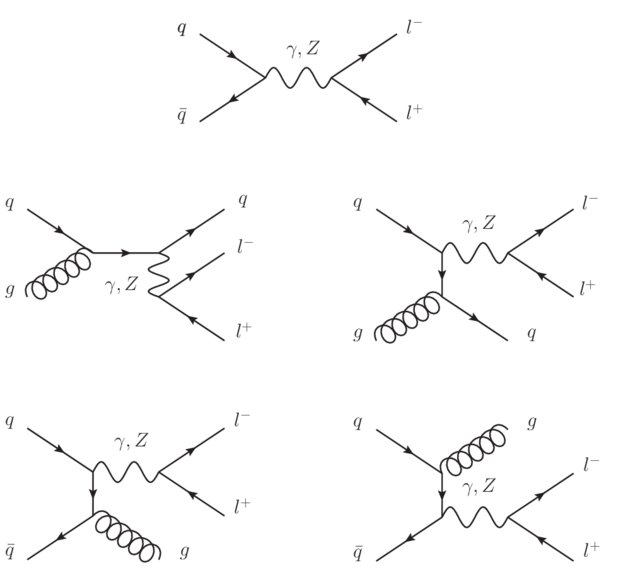
\includegraphics[height =
  6cm]{Figures/c4/dia/The-Feynman-graphs-for-Drell-Yan-pair-production-at-the-Oa-and-Oaa-s-orders_W640.jpeg}
\hspace{1cm}
  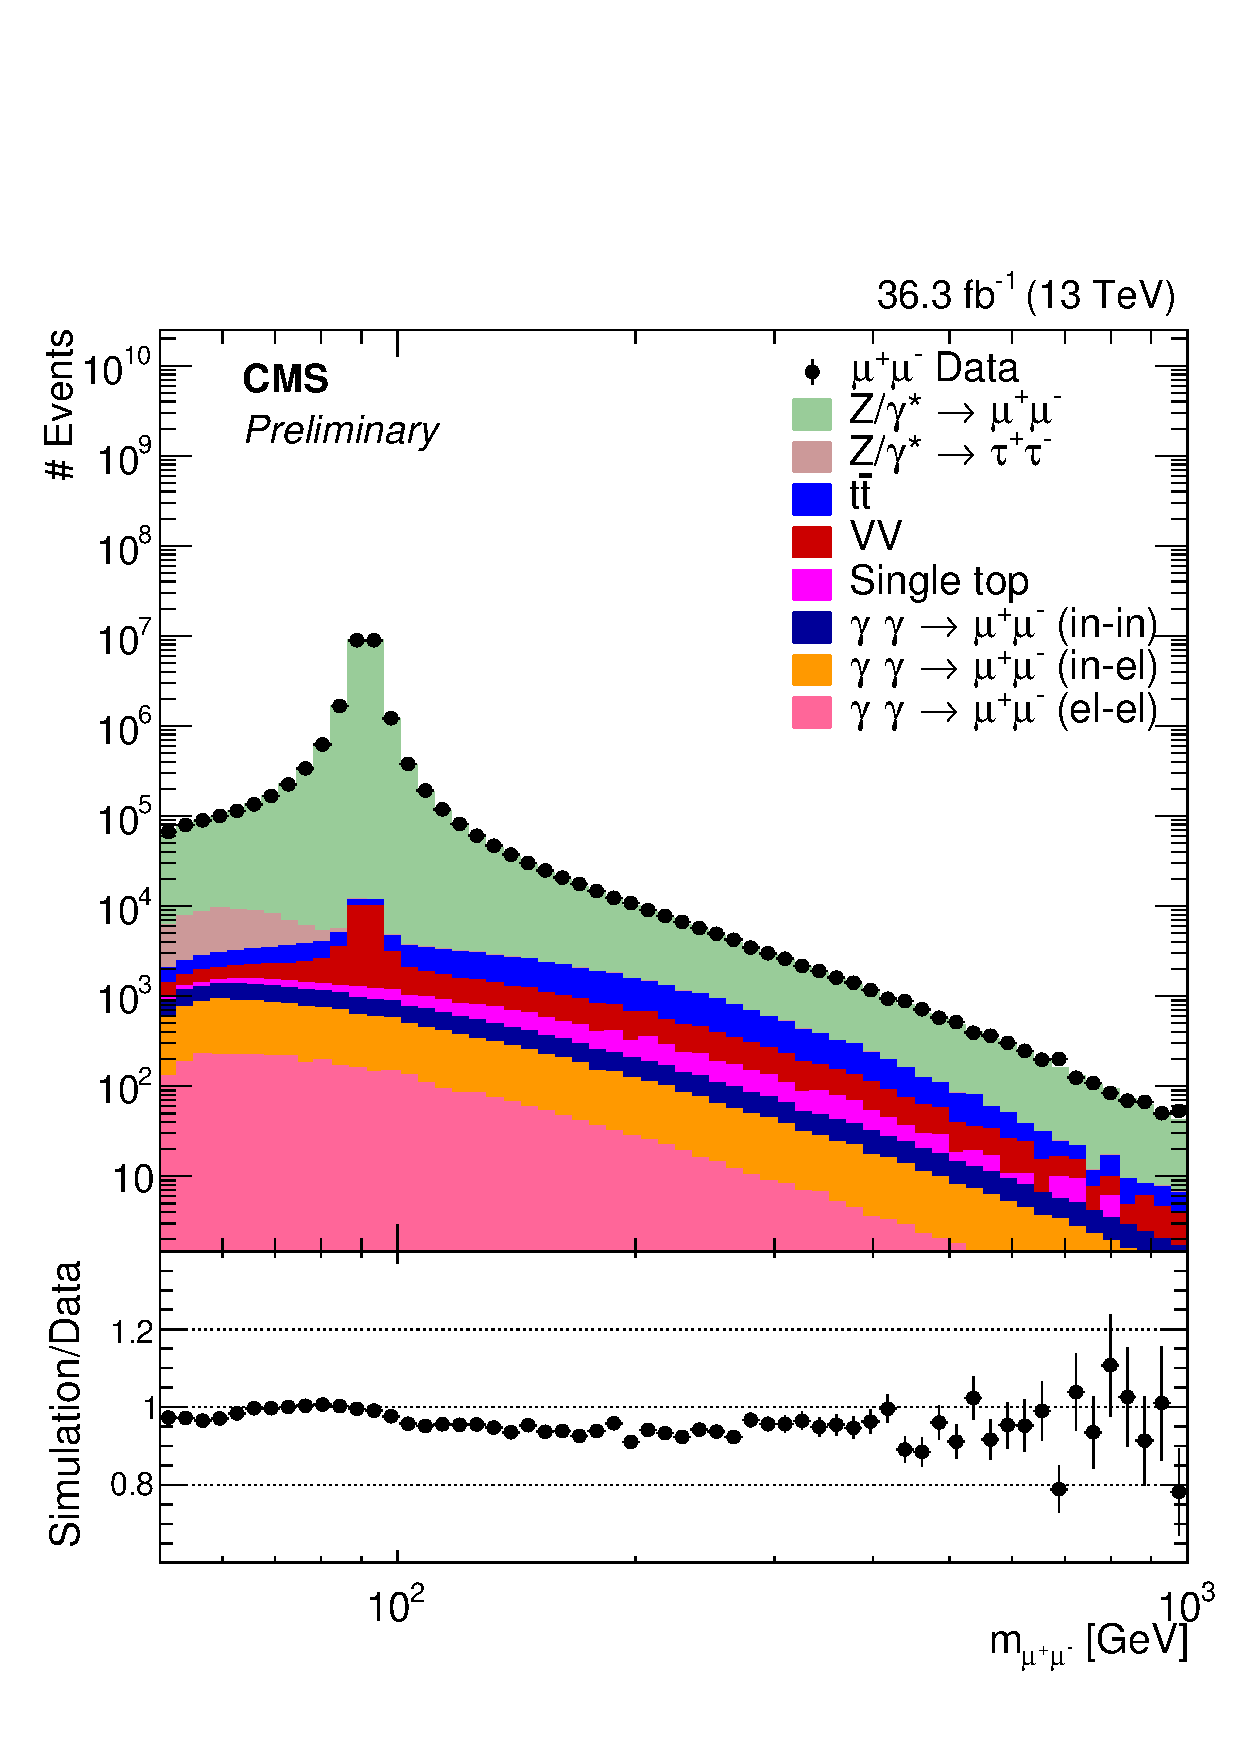
\includegraphics[height = 6cm]{Figures/c4/dia/Figure_001-a.pdf}
  \caption{On the left, the typical DY production
    diagrams~\cite{diagram}. On the right, distributions of the
    invariant mass, $M_{\mu \mu}$, of dimuon events. The \PZ resonance
    is clear at $M=91.2$\GeV~\cite{CMS-PAS-SMP-20-003}.}
  \label{fig:c44}
\end{figure}
Drell-Yan events contribute in three prompt leptons final states when
associated with a jet production (DY plus jets) or when one nonprompt
lepton is reconstructed and passes the analysis selection. The Drell-Yan
production cross section is so large with respect to other three
leptons processes that even a modest misidentification probability can
lead to a large background contribution.

\paragraph{Top quark production.}\label{sec:c4ttbar}
In both the analysis presented in the following two chapters, the
background from top quark production ($t\bar{t}$) is among the
dominant ones. \\
In this case, the three leptons come from $t\bar{t}$ production 
where they originate from semi-leptonic b quark decay and lepton \PW decay.

\begin{figure}[h!]
\centering
 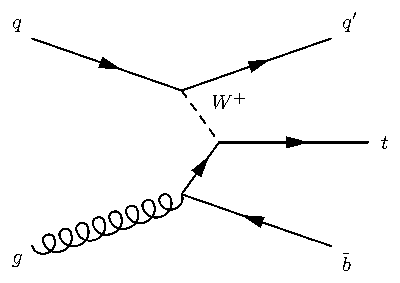
\includegraphics[width=0.25\textwidth]{Figures/c4/dia/60100003.pdf}
  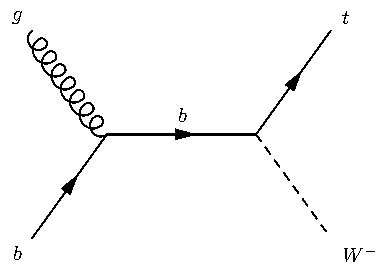
\includegraphics[width=0.25\textwidth]{Figures/c4/dia/60100001.pdf}\\
  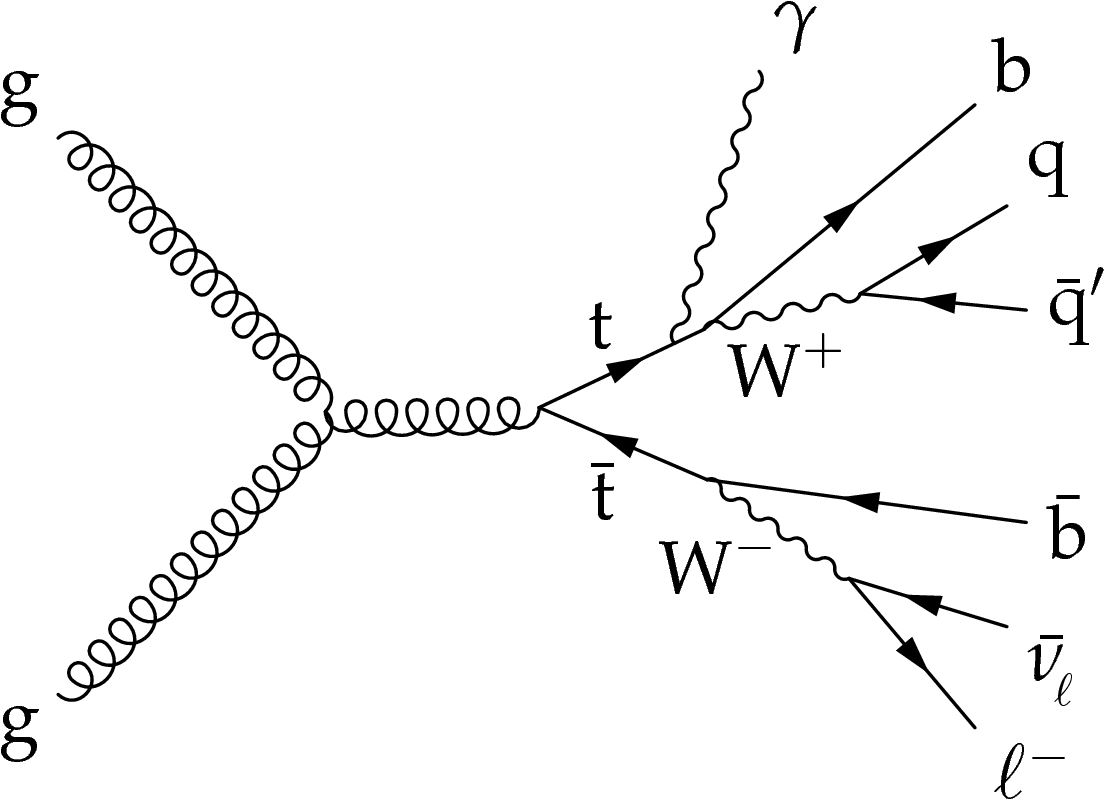
\includegraphics[width=0.4\textwidth]{Figures/c4/dia/Figure_001-a_tt.png} 
  \caption{Diagrams for single top production and $t\bar{t}$ production.~\cite{diagram}}
  \label{fig:c46}
\end{figure}


\subsection{Long-lived particles}\label{sec:c4LLbgk}
The analysis presented in Chapter~\ref{Chapter6} looks for displaced
vertices and displaced leptons produced relatively far from the PV.
This kind of signature happens to be very different with respect the
very well known SM processes. Along these lines, the backgrounds
are not the conventional ones and
therefore special care has to be used in understanding them.\\
In Figure~\ref{fig:c4LLbgk} the phase space of long-lived HNLs is
superimposed with potentially important backgrounds coming from
long-lived meson decays. The figure shows the crowded area as function
of HNL mass and life time.

\begin{figure}[h!]
\centering
 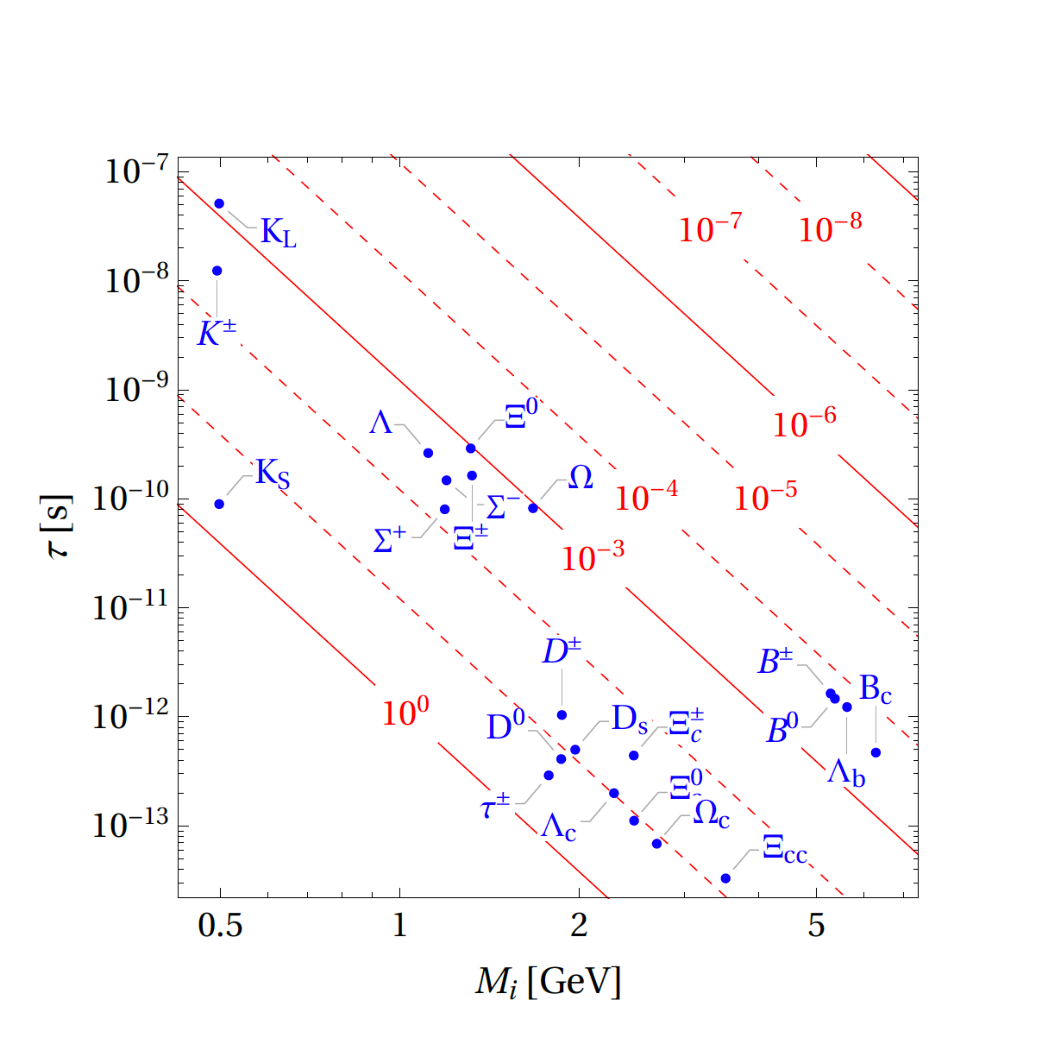
\includegraphics[clip,trim=0.5cm 0.5cm 2cm 2cm, width=0.7\textwidth]{Figures/c4/resonances.pdf}
  \caption{HNL \mixpar (red lines) superimposed with potentially important SM backgrounds
(blue dots) as function of HNL mass and life time~\cite{Drewes_2020_jan}.}
  \label{fig:c4LLbgk}
\end{figure}

As is evident from Figure~\ref{fig:c4LLbgk}, the resonance and
meson backgrounds can be rejected with proper selection criteria on
the invariant mass of the decay products and on
the displacement. This strategy will be presented in
Chapter~\ref{Chapter6} where carefully selected mass windows are removed
to avoid background contamination.




\clearpage
\section{Heavy Neutrino signal event Generation}\label{sec:c4hnl}
This section is strictly relevant to the signal model used in
Chapters~\ref{Chapter5} and~\ref{Chapter6}. The model is circumscribed to the
CMS results only and it is not adopted for ATLAS's
results(~\cite{atlasintro2}) which are often used for comparison
purposes with the CMS results.



\subsection{Signal simulation}\label{sec:c4hnlmodel}

Signal samples are generated using the
\texttt{MadGraph5\_aMC@NLO}~\cite{Alwall_2014} software. 
For the prompt HNL
model a generator is used with next-to-leading order (NLO) precision
in perturbative quantum chromodynamics; for the long-lived model, it
is adopted a leading order (LO) precision in the strong
coupling constant $\alpha_{\mathrm{S}}$.\\
The generation is based on the \texttt{heavyN} model described in
Ref.~\cite{Atre:2009rg}, which is available in Universal FeynRules
Output (UFO) by Ref.~\cite{Alva:2014gxa,Degrande_2016,heavyN}.
This model extends the SM with up to three RH neutrinos,
which are singlets under the SM gauge symmetry.
The mass and mixing parameters of the HNL can be defined for each
scenario to probe.

The HNL production is simulated via charged current (CC) Drell-Yan
process,~\ref{fid:hnl_production}(a), via gluon
fusion,~\ref{fid:hnl_production}(b), and via $\PW \gamma$
fusion,~\ref{fid:hnl_production}(c). 
\begin{figure}[h!]
\centering
 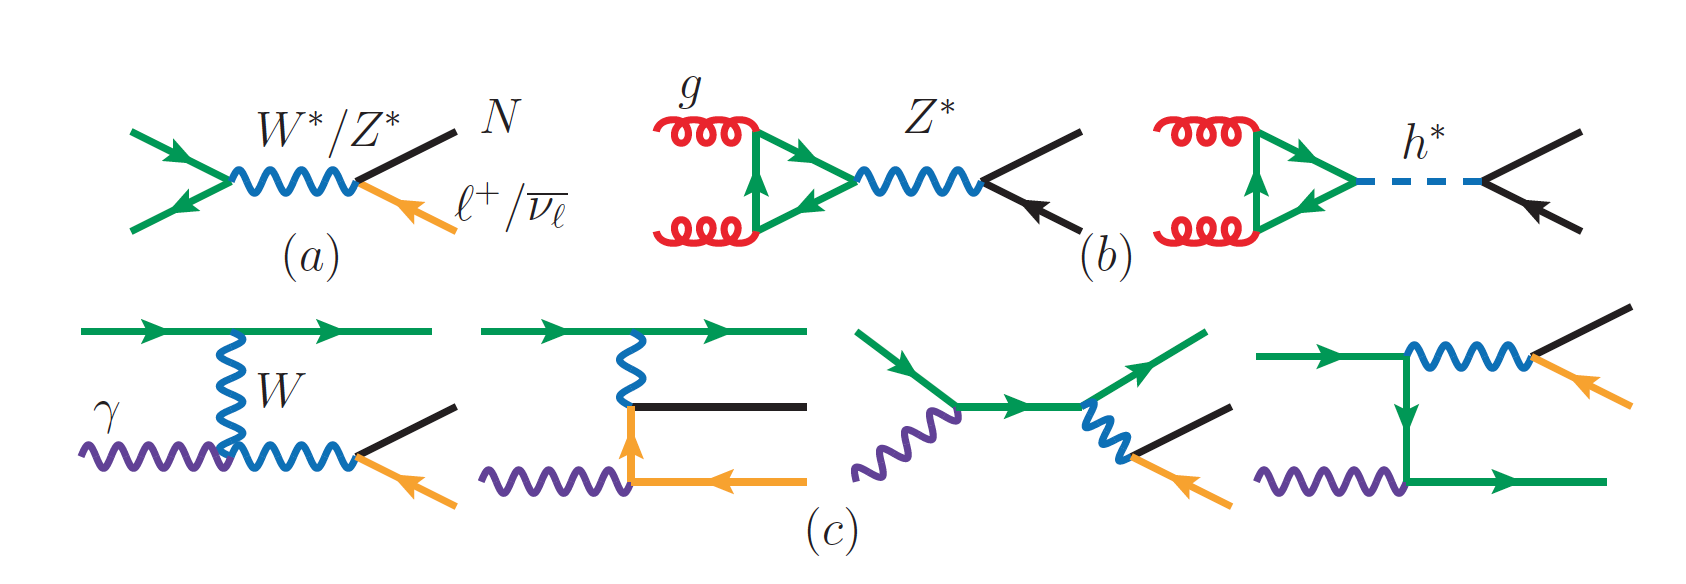
\includegraphics[clip,trim=0cm 0cm 0cm 1cm, width=0.70\textwidth]{Figures/c4/hnl_production}
  \caption{Diagrams for heavy neutrino production mechanisms at LHC~\cite{Pascoli_2019}}
  \label{fid:hnl_production}
\end{figure}

The production mechanisms via gluon and vector-boson fusion are
crucial because
\begin{wrapfigure}{r}{0.48\textwidth}
  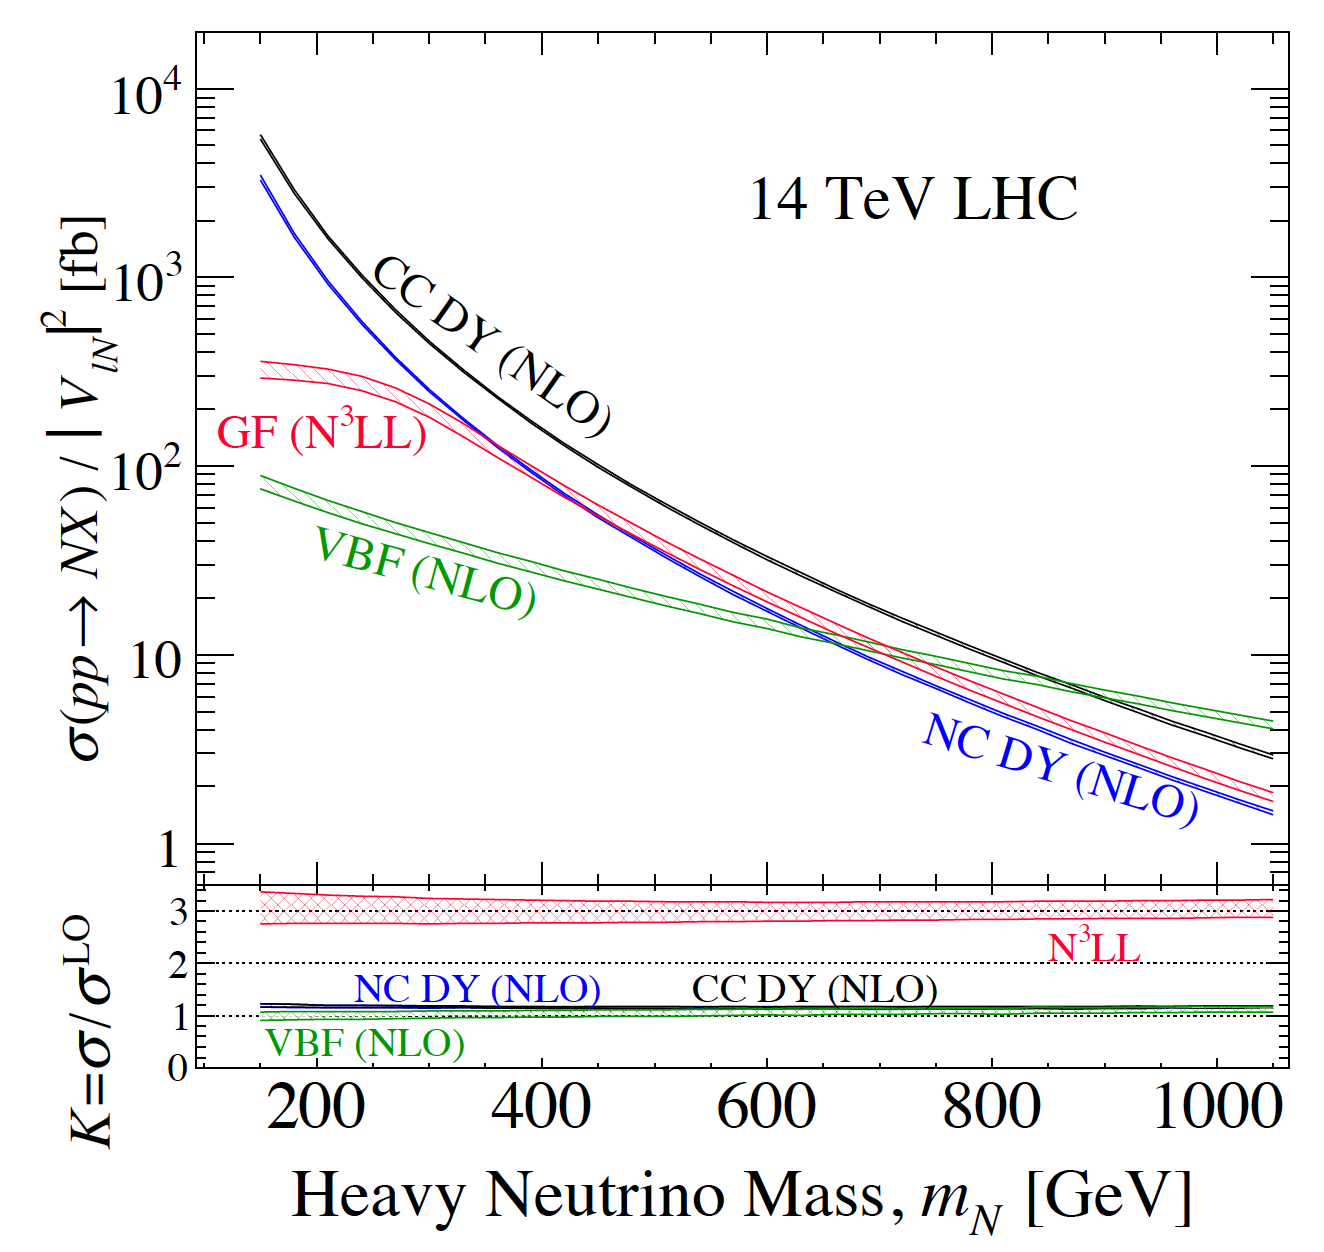
\includegraphics[clip,trim=0cm 0cm 0.5cm 0.5cm, width=.39\textwidth]{Figures/c4/hnl_lhc_production}
  \caption{``HNL production cross section, divided by \mixpar, via
charged (CC) and neutral (NC) current DY, $\PW \gamma$ fusion (VBF),
and gluon fusion (GF) at $\sqrt{s}
\sim 14$\TeV ''~\cite{Pascoli_2019}.}
  \label{fig:hnl_lhc_graph}
\end{wrapfigure} 
 at the energies the LHC operates and at high \hnl mass the CC DY process
is no longer the only viable way for producing heavy neutrinos. 
Vector boson fusion $\PW \gamma \rightarrow N
\ell^{\pm}$~\cite{PhysRevLett.112.081801, Alva:2014gxa,Degrande_2016}
is the dominant production mechanism at the LHC 
energies for HNLs with very large masses
(TeV energy scale)~\cite{Alva:2014gxa,Degrande_2016, Pascoli_2019} and for
lighter HNLs it enhances the inclusive production rate. Neutral current
processes~\cite{PhysRevD.44.1593,WILLENBROCK1985429} which include
gluon fusion, $gg \rightarrow \PZ^{*}/H^{*} \rightarrow \hnl \nu \ell$
can even surpass CC DY cross section for large HNL masses~\cite{PhysRevD.96.055042,
  Pascoli_2019}. Refer to Figure~\ref{fig:hnl_lhc_graph} for
references.\\
For the high mass \hnl samples made for the search described in
Chapter~\ref{Chapter5}, both gluon
fusion and $\PW \gamma$
fusion are added as production mechanisms. 
The first two employ
the NNPDF3.0 NLO PDFs set~\cite{Ball_2015}, while $\PW \gamma$
fusion uses the LUXqed plus PDF4LHC15 NNLO 100
PDF set~\cite{PhysRevLett.117.242002}.\\
For all the signal MC samples the parton showering and hadronization are simulated with PYTHIA. \\

For signal simulation, samples with HNLs masses from 
$\mhnl = 1$\GeV to $\mhnl = 1.2$\TeV are produced. The simulated HNL couple
exclusively to one of the three SM neutrino families with different
mixing probabilities, typically in a range $\mixpar = 10^{-6}$ -- 1,
depending on the mass. The mixing parameters are:
\begin{linenomath}
\begin{equation}
  \mathbf{V}_{\hnl\ell} =
  \begin{pmatrix}
    \mathrm{V}_{\hnl\Pe} & 0 & 0 \\
    0                   & 0 & 0 \\
    0                   & 0 & 0 \\
  \end{pmatrix},
%% \end{equation}
\quad\quad
%% \begin{equation}
  \mathbf{V}_{\hnl\ell} =
  \begin{pmatrix}
    0                    & 0 & 0 \\
    \mathrm{V}_{\hnl\PGm} & 0 & 0 \\
    0                    & 0 & 0 \\
  \end{pmatrix},
%% \end{equation}
\end{equation}
\end{linenomath}
where $\mathbf{V}_{\hnl\ell}$ represents the active-sterile neutrino
mixing matrix:
\begin{linenomath}
\begin{equation}
  \begin{pmatrix}
    \nu_{\Pe}  \\
    \nu_{\PGm} \\
    \nu_{\PGt} \\
  \end{pmatrix} ~=~
  \mathbf{V}_{\hnl\ell}\,\cdot\,
  \begin{pmatrix}
    \hnl_{1} \\
    \hnl_{2} \\
    \hnl_{3} \\
  \end{pmatrix}.
\end{equation}
\end{linenomath}

\begin{figure}[h!]
\centering
 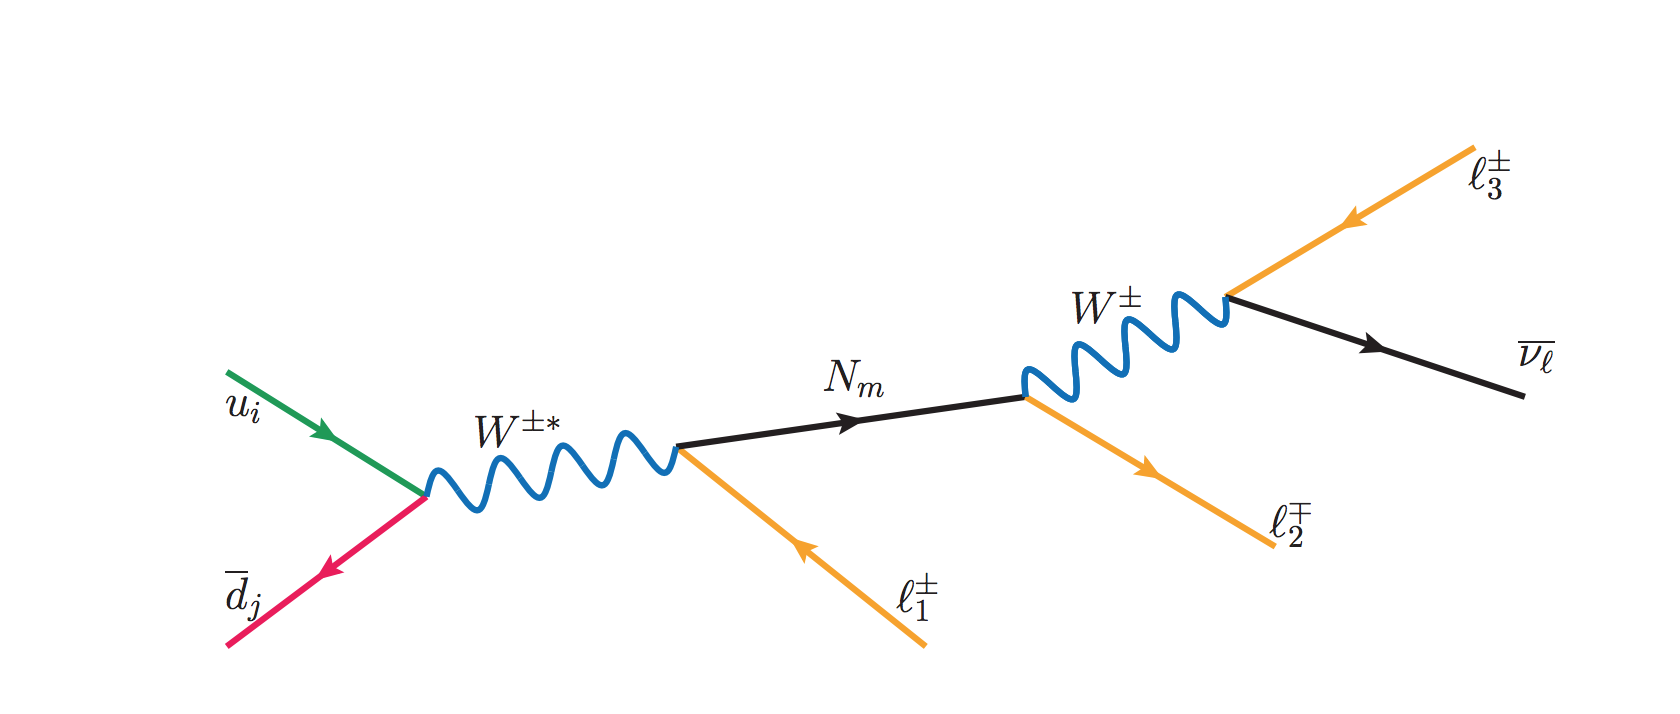
\includegraphics[clip,trim=0.5cm 0.5cm 0.5cm 2.5cm, width=0.75\textwidth]{Figures/c4/hnl_graph}
  \caption{HNL production and decay. Only the leptonic decay of the \PW considered~\cite{Pascoli_2019}.}
  \label{fig:c46}
\end{figure}


\subsubsection{Long-lived HNL samples}\label{sec:reweighting}
For the long-lived HNL, the width $\Gamma_{\hnl}$ is computed automatically by the
generator, and the mean lifetime $\tau_{\hnl} = \hbar/\Gamma_{\hnl}$
is used to extract the HNL lifetime in each simulated event,
according to a decay probability distribution
\begin{linenomath}
  \begin{equation}
\frac{dN(t)}{dt} = \frac{1}{\tau_{\hnl}}e^{-t/\tau_{\hnl}}
  \end{equation}
  \label{eq:dndt}
\end{linenomath}
where $t$ is the
\emph{proper} lifetime, measured in the HNL rest frame.

As explained in Section~\ref{sec:promptll}, the values of \mhnl
and \mixpar do not only determine the HNL production cross section,
but also its mean lifetime and, consequently, its kinematics,
acceptance, and reconstruction efficiency.
For a fixed value of \mhnl, therefore, a simple cross section
rescaling is not sufficient to correctly reproduce the behavior of
other HNLs with same mass and different \mixpar.

The simple and naive approach with endless computing power would be an
iterative one. For a \mhnl
and \mixpar scenario, first compute the limits by evaluating parameters
of interest as the overall \emph{signal strength} (number of signal events /
number of expected signal events); when computing the fit between
signal, data and background yields, by default the signal strength is
left floating in the fit, so that the measurement is independent from the
presence or absence of a signal. Depending on the value of the signal
strength there are two options. If the signal strength is below 1 it
means that the \mhnl --\mixpar case is excluded and a new sample with
same \mhnl but smaller \mixpar has to be simulated. If the signal strength is above 1 it
means that the analysis is not sensitive to that \mhnl --\mixpar case and a new sample with
same \mhnl but larger \mixpar has to be simulated. This iteration can
be repeated with steps smaller and smaller until the signal strength is
exactly 1 which means we found the exclusion limits. It is clear that
this kind of approach is not sustainable due to the limited computing
time and power available. A smarter correction procedure is needed.

To this purpose, it is used instead a per-event re-weighting technique
based on the HNL lifetime, which properly accounts for all the
variations in kinematics and acceptance.
First, it is noticed that the average kinematics of a HNL decay
is entirely defined by the HNL mass \mhnl, its momentum
$p_\hnl=\beta\gamma\mhnl$, and its decay length,
independently of its mean lifetime $\tau_\hnl$.
Therefore, given a simulated HNL sample of mass \mhnl
and mean lifetime $\tau_0$, we can reproduce the kinematic
distributions of any target HNL scenario with same mass and 
different lifetime, $(\mhnl, \tau_{\mathrm T})$.
An event with proper decay time $t$ taken from the simulated sample
of mean lifetime $\tau_0$ is re-weighted by the ratio of
probabilities to obtain $t$ from $\tau_{\mathrm T}$ or from $\tau_0$:
\begin{linenomath}
  \begin{equation}
    W(t; \tau_0\to\tau_{\mathrm T}) ~=~ \frac{dN_{\mathrm T}(t)/dt}{dN_0(t)/dt} ~=~
    \frac{\tau_0}{\tau_{\mathrm T}}\exp{\left[-t\left(\frac{1}{\tau_{\mathrm T}}-\frac{1}{\tau_0}\right)\right]}.
  \label{eq:ctauReweightingSingle}
  \end{equation}
\end{linenomath}
Furthemore, it can be used a set of multiple HNL samples with different lifetimes
$\{\tau_i\}$ to emulate the $\tau_{\mathrm T}$ scenario. In this case the
decay time distributions must include the correct normalization
factors for each sample, $N_i/\tau_i$, where $N_i$ is the number of
simulated events for the sample with mean lifetime $\tau_i$ and
$N_{\mathrm{tot}} = \sum_i N_i$:
\begin{linenomath}
  \begin{equation*}
    W(t; \{\tau_i\}\to\tau_{\mathrm T}) ~=~ \frac{dN_{\mathrm T}(t)/dt}{\sum_i dN_i(t)/dt} ~=~
    \frac{\frac{N_{\mathrm{tot}}}{\tau_{\mathrm{T}}}\exp{(-t/\tau_{\mathrm{T}})}}
         {\sum_i\frac{N_{i}}{\tau_i}\exp{(-t/\tau_i)}}.
  %\label{eq:ctauReweightingMult}
  \end{equation*}
\end{linenomath}
If $\sigma_{\mathrm{T}}$ is the production cross section for
$(\mhnl,\tau_{\mathrm T})$ and $\mathcal{L}$ is the integrated luminosity,
the complete event weight is
\begin{linenomath}
  \begin{equation}
    w(t; \{\tau_i\}\to\tau_{\mathrm T}) ~=~
    \frac{\sigma_{\mathrm{T}}\mathcal{L}}{N_{\mathrm{tot}}}\,W(t;\{\tau_i\}\to\tau_{\mathrm T})
     ~=~ \frac{\frac{\sigma_{\mathrm{T}}\mathcal{L}}{\tau_{\mathrm{T}}}\exp{(-t/\tau_{\mathrm{T}})}}
         {\sum_i\frac{N_{i}}{\tau_i}\exp{(-t/\tau_i)}}.
  \label{eq:ctauReweighting}
  \end{equation}
\end{linenomath}
Figure~\ref{fig:newReweightGen} compares the proper decay length $ct$
distributions for three samples of $\mhnl=4$\GeV and different mean
lifetimes, and the corresponding models built from the sum of the
three samples by re-weighting with Eq.~\ref{eq:ctauReweighting}. An
excellent agreement is observed, with the re-weighted summed sample
exhibiting less statistical fluctuations than the individual samples.
\begin{figure}[h!]
  \centering
  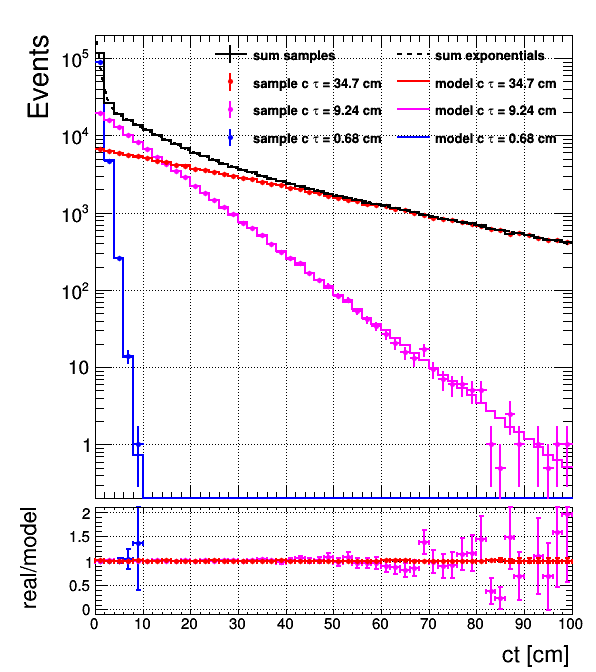
\includegraphics[width = .55\textwidth]{Figures/c4/reweighting/ctau_genLevel_unskimmed.png}
  \caption{Distribution of the proper decay length $ct$ for three HNL
    samples of $\mhnl=4\GeV$ and different mean lifetimes (points withs
    error bars),
    and the corresponding models built from the sum of the three
    samples by re-weighting with Eq.~\ref{eq:ctauReweighting}
    (continuous histograms). The black, continuous histogram shows the
    sum of the three samples, while the black, dashed line is the sum
    of the three exponential functions that describe the proper decay
    length of the three samples. \dani}
  \label{fig:newReweightGen}
\end{figure}


Figure~\ref{fig:newReweightRec} shows distributions of the
reconstructed dilepton mass (\mtwol) and secondary-vertex transverse
displacement (\Deltwod (~\ref{sec:c2IP})) for a HNL scenario with
$\mhnl=4$\GeV and $\mixparm = 6.31\cdot 10^{-6}$ in 2018,
modeled using either a single sample with the re-weighting of
Eq.~\ref{eq:ctauReweightingSingle} (black histograms), or the sum of
three samples with different $\mixparm$ values and the re-weighting of
Eq.~\ref{eq:ctauReweighting} (red histograms). The two models are compatible.\\
The histograms
presented in Figure~\ref{fig:newReweightRec} are filled with events
which pass the event selection specifically designed for the
long-lived analysis presented in Chapter~\ref{Chapter6}, for details
refer to Section~\ref{sec:llanalisi}. 


\begin{figure}[h!]
  \centering
  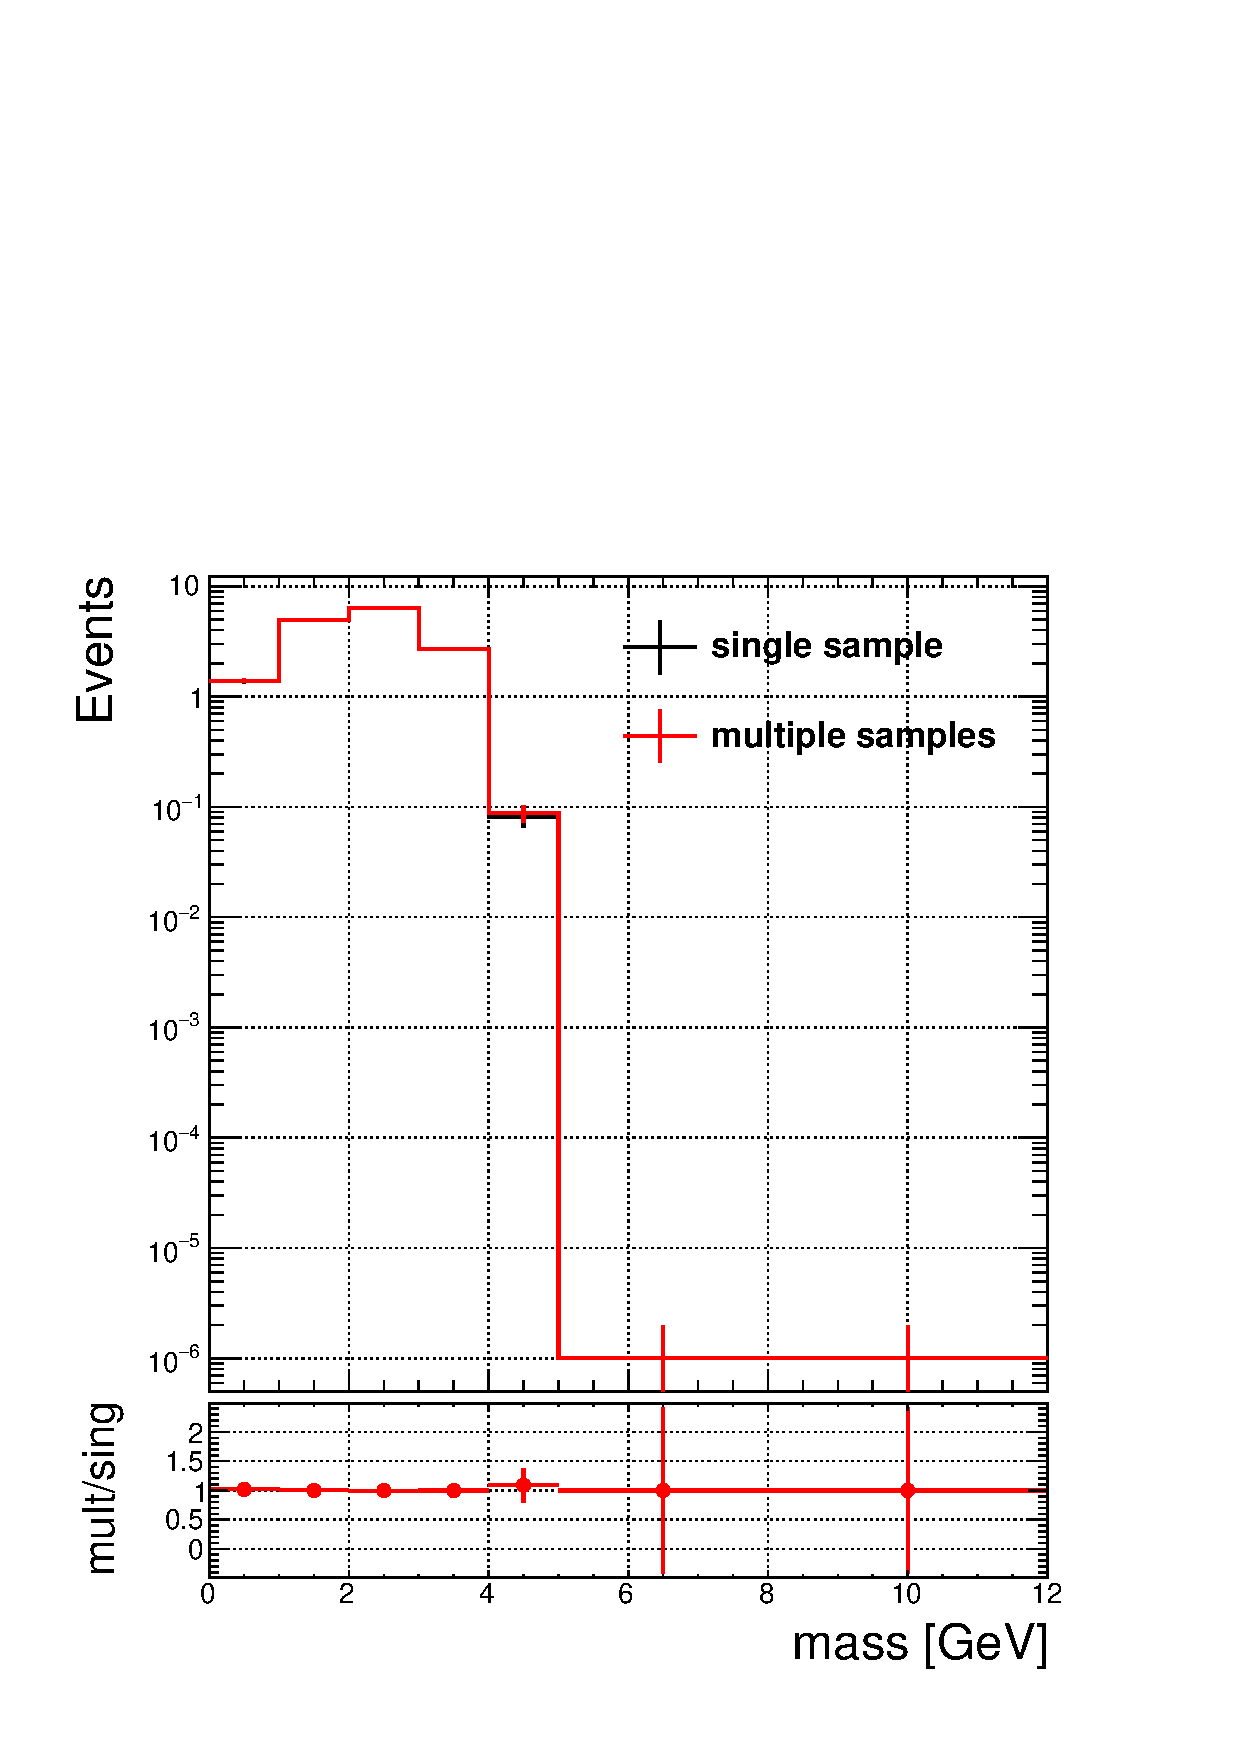
\includegraphics[width = .32\textwidth]{Figures/c4/reweighting/reweighting_mass_M4p0_V0p00251197_mu_18.pdf}
  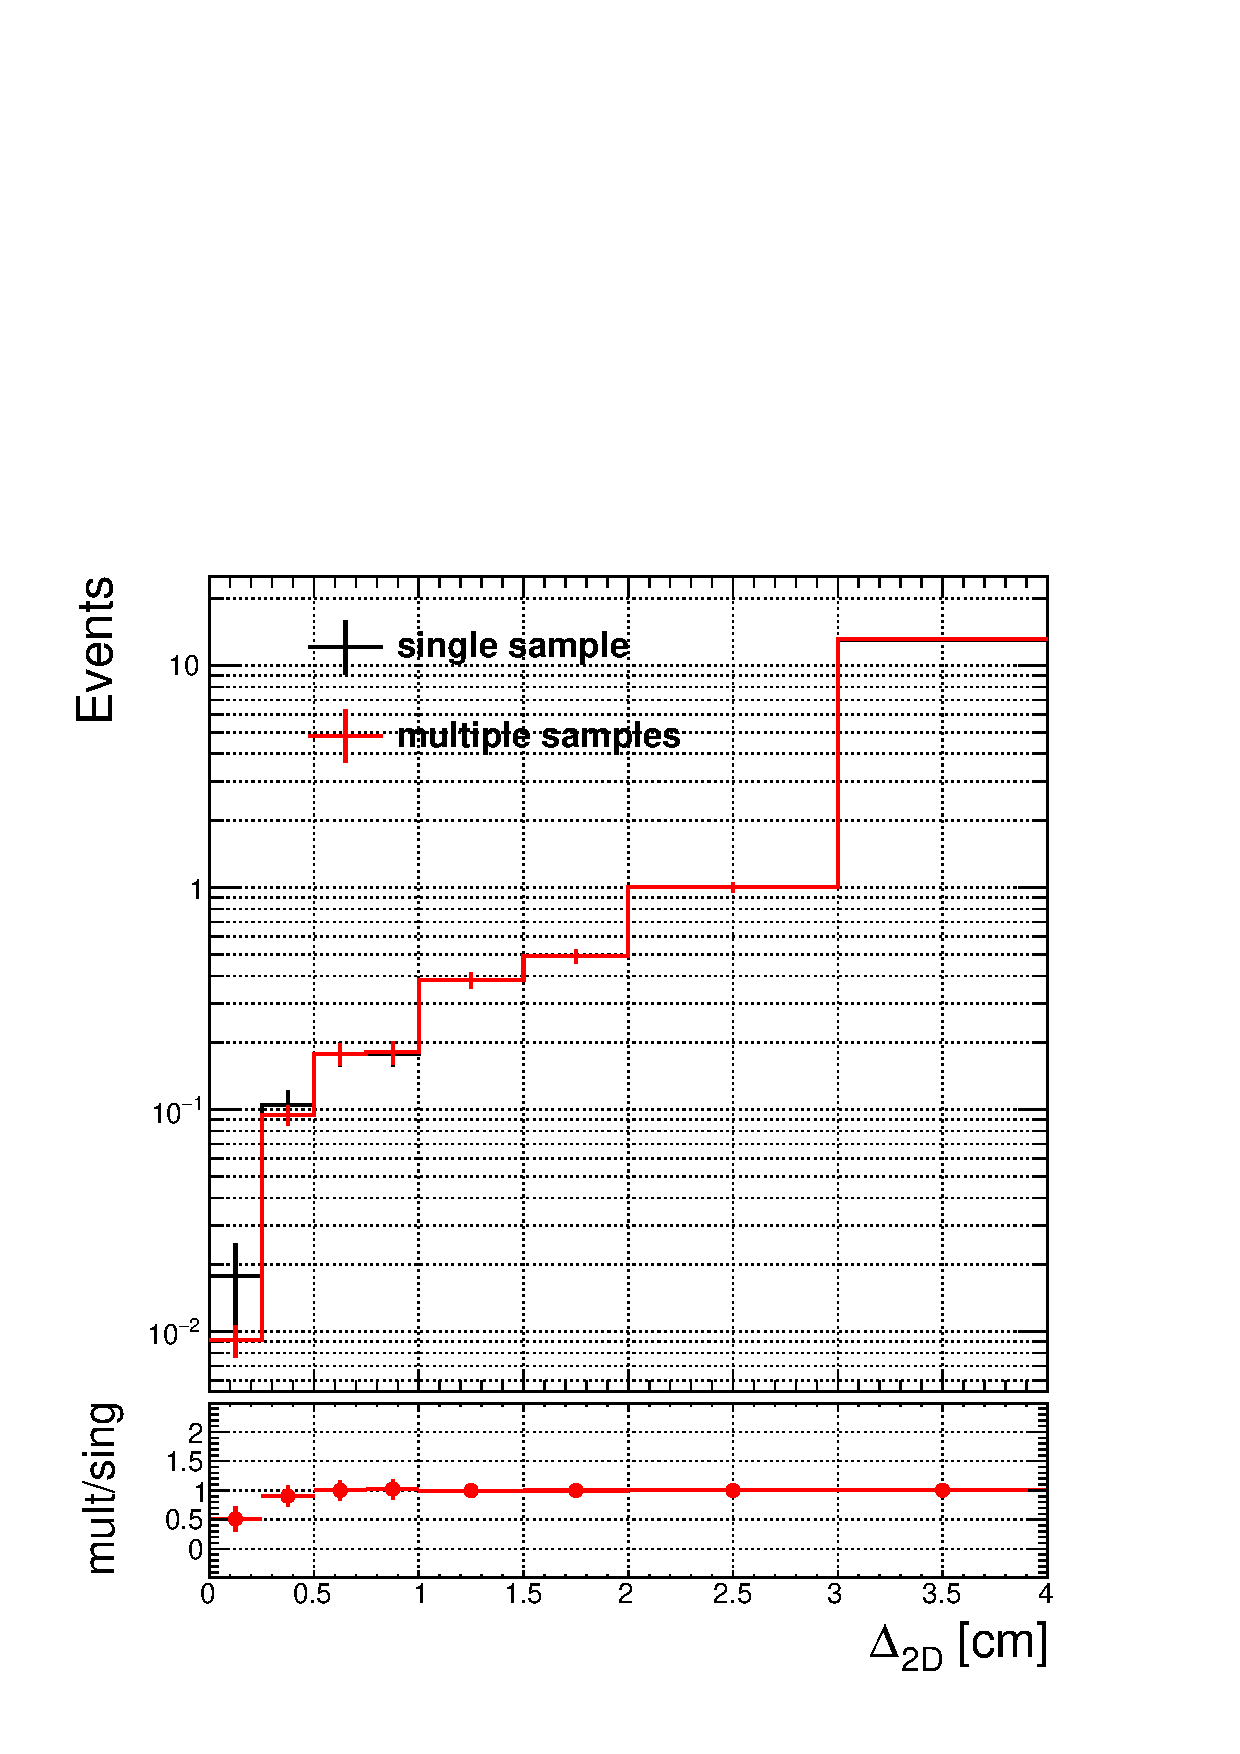
\includegraphics[width = .32\textwidth]{Figures/c4/reweighting/reweighting_disp_M4p0_V0p00251197_mu_18.pdf}
  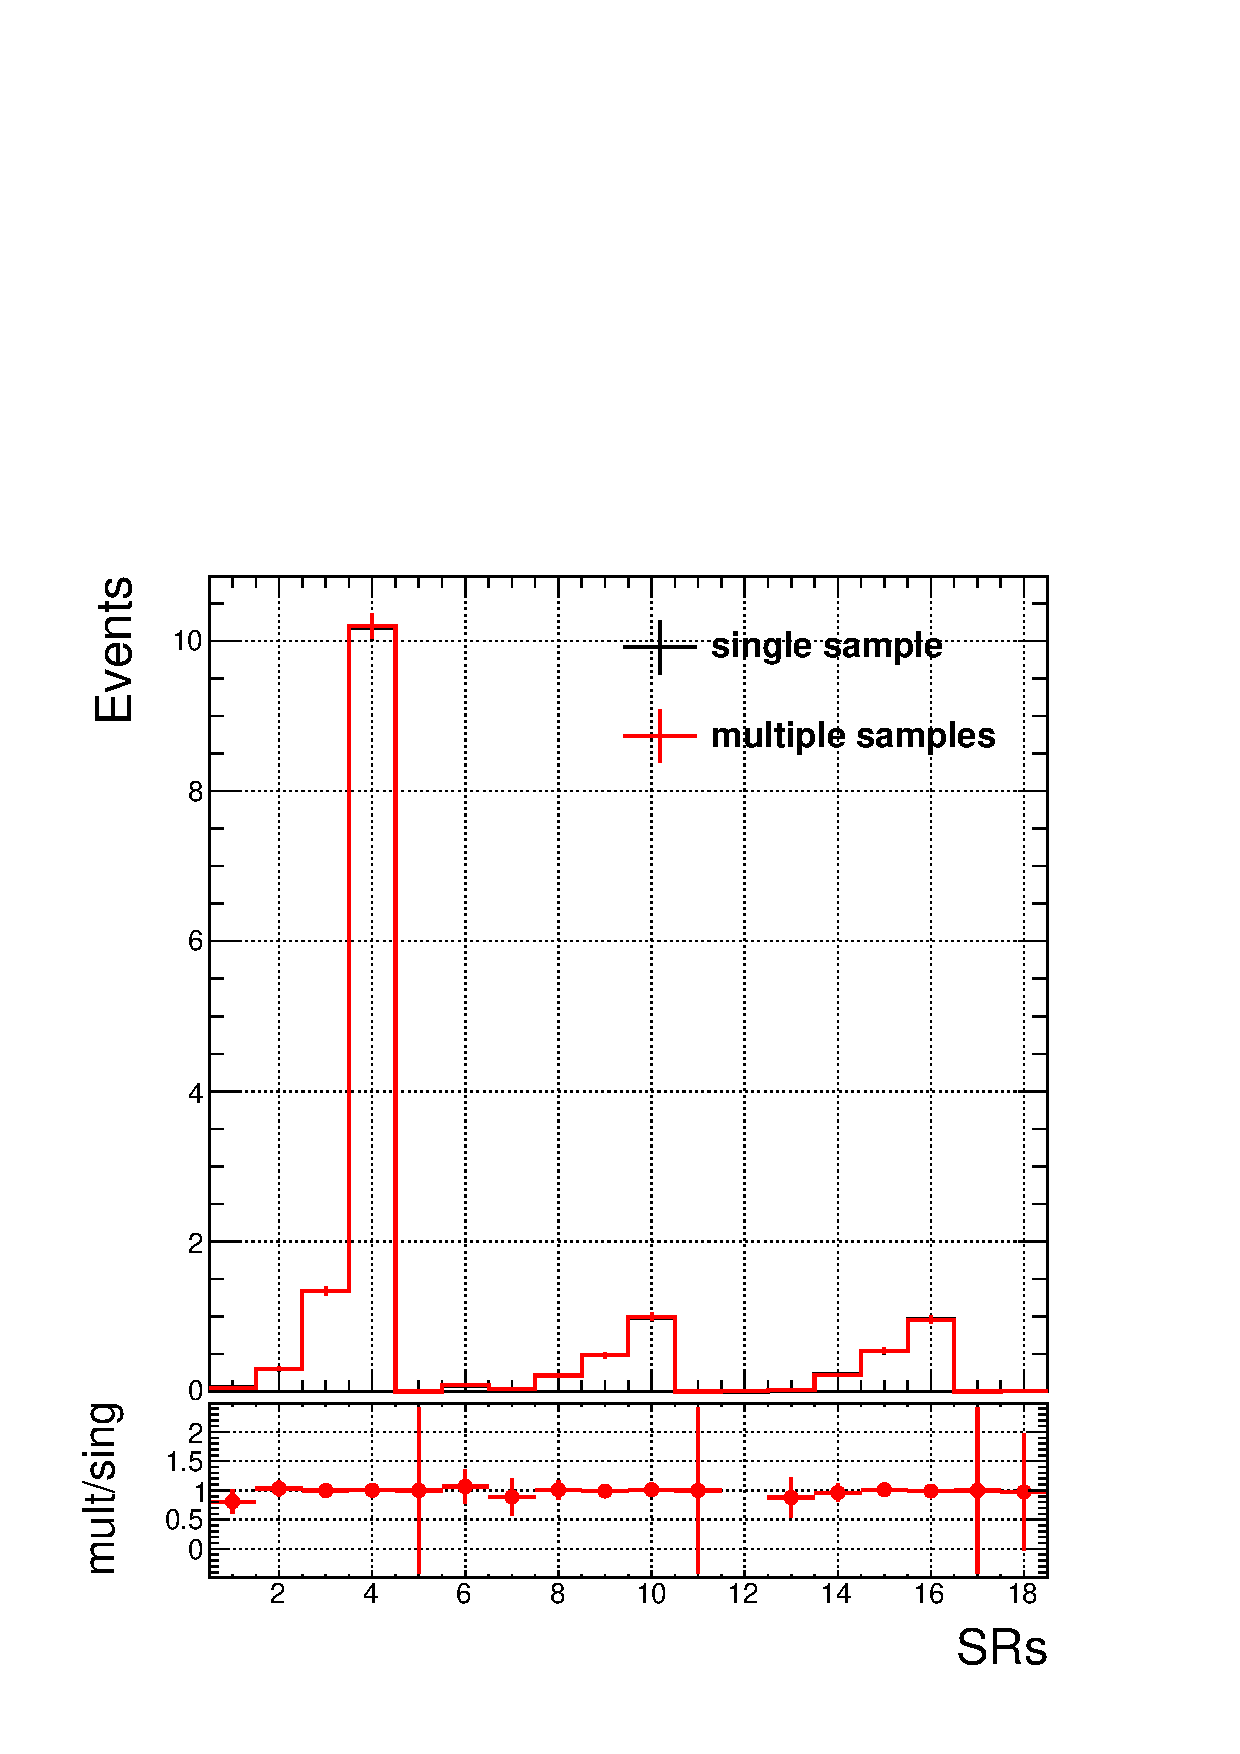
\includegraphics[width = .32\textwidth]{Figures/c4/reweighting/reweighting_M4p0_V0p00251197_mu_18.pdf}
  \caption{Distributions of the reconstructed dilepton mass \mtwol
    (left), secondary-vertex transverse displacement \Deltwod (middle), and final signal-region yields described in
    Section~\ref{sec:llbaselinesel} (right), for a HNL scenario with
    $\mhnl=4\GeV$ and $\mixparm = 6.31\cdot 10^{-6}$ in the 2018
    simulation. The black histograms are modeled
    using a single sample with the re-weighting of
    Eq.~\ref{eq:ctauReweightingSingle}, while the red histograms use
    the sum of three samples with different $\mixparm$ values and the
    re-weighting of Eq.~\ref{eq:ctauReweighting}. \dani}
  \label{fig:newReweightRec}
\end{figure}



\subsubsection{Dirac HNL signal emulation}\label{sec:c4diracmajo}
The HNL production cross section is fixed by the \mhnl and \mixpar
values~\cite{Degrande_2016,heavyN}, and it is the same for Dirac and
Majorana HNLs.
The resonance width for a Majorana HNL, on the other hand, is exactly
twice the width of a Dirac HNL with same \mhnl--\mixpar values, due to
the additional charge-conjugated (LNV) decay channels (refer to Figure~\ref{fig:dirac_majo}).
As a consequence, the average lifetime of a Dirac HNL is twice that of
a Majorana HNL with same $(\mhnl,\mixpar)$. Refer
to Section~\ref{sec:c3majo_dirac}.
\begin{figure}[h!]
\centering
 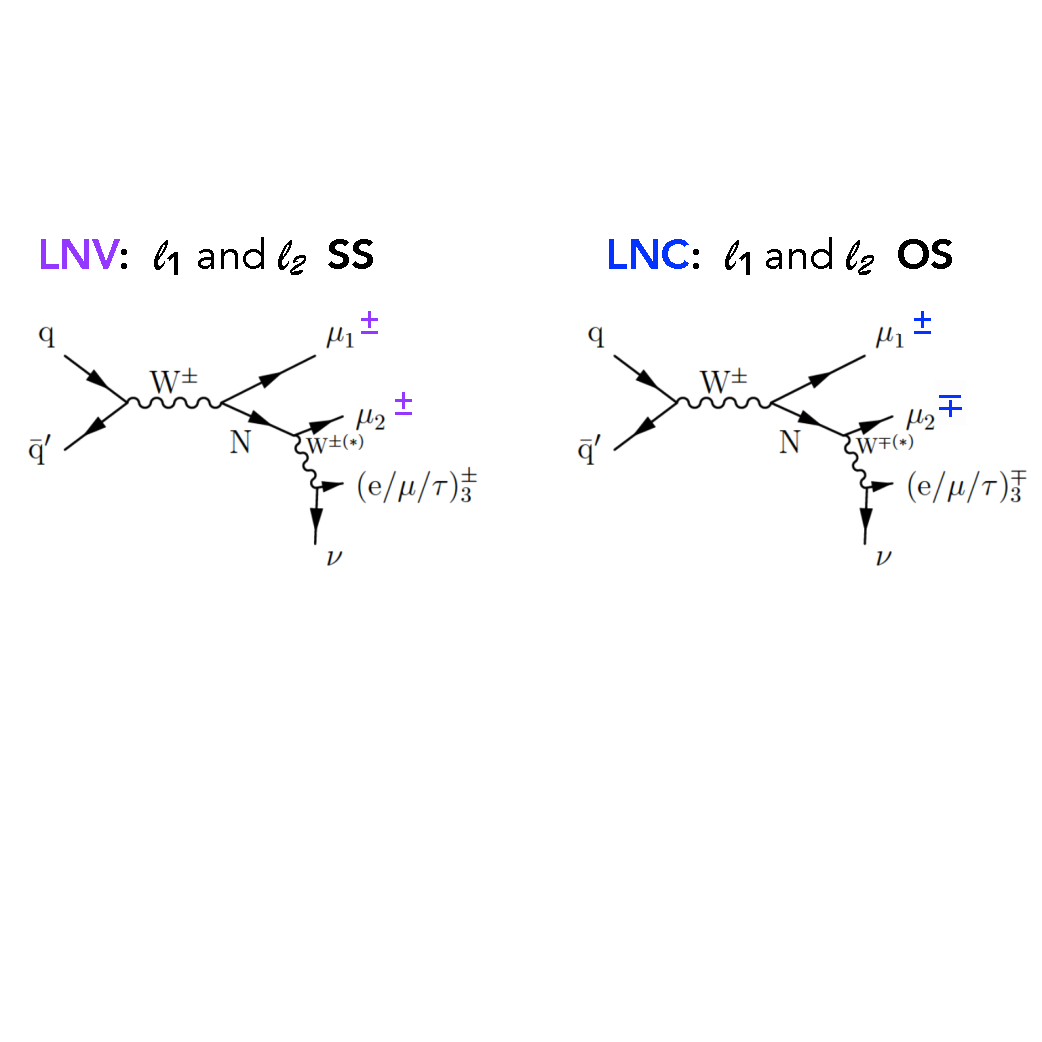
\includegraphics[clip,trim=0cm 7cm 0cm 3cm, width=0.65\textwidth]{Figures/c4/dirac_majo2}
  \caption{Visualization of the LNV and LVC cases. Majorana HNLs
    can decay in both cases while Dirac HNLs can only have LNC decay.}
  \label{fig:dirac_majo}
\end{figure}

For the prompt analysis (Chapter~\ref{Chapter5}) there is no 
need to produce distinct Dirac and Majorana MC samples since there is
no difference between them except the final state combinations. For the
long-lived scenario separate samples are necessary.

After the lesson learned with the emulation procedure described 
above in Section~\ref{sec:reweighting}, a similar idea and strategy
was also adopted for the Dirac-Majorana case.\\
To optimize computing resources and in the interest of time,
high-statistics MC samples were produced on a large scale for Majorana
HNL scenarios only.
Dirac HNL scenarios for any $(\mhnl,\mixpar)$ point were emulated
starting from the corresponding Majorana HNL samples, following these
steps:
\begin{itemize}
\setlength\itemsep{-0.2em}
\item from a Majorana HNL sample, select only the LNC events by
  looking at the unique ID number of the generated particles;
\item re-weight each LNC event to emulate the correct lifetime of the
  Dirac HNL, by using Eq.~\ref{eq:ctauReweightingSingle} with
  $\tau_{\mathrm{T}}=2\tau_0$;
\item since only half the events of the original Majorana sample are
  used (while the cross section is the same for Majorana and Dirac
  scenarios), add a factor 2 to the event weight to restore the correct
  normalization.
\end{itemize}
This method provides a good modeling of the Dirac HNL signal, but
uses only half the events from the Majorana HNL MC samples. With a
simple extra assumption, it is possible to make use of the full
statistical power of our MC production.

As explained in the Section~\ref{sec:llresults}, the signal selection is the
same for LNC and LNV events. Just in the final stage of the analysis,
events are split into same-lepton-charge and opposite-lepton-charge
categories to distinguish LNV and LNC events for the physics
interpretation. If we assume that the lepton efficiency and
acceptance are the same for positively and negatively charged leptons
(\ie, same reconstruction and identification efficiency, same momentum
scale and resolution, etc.), then we can use both LNC and LNV events
from the Majorana HNL samples to emulate the Dirac scenarios, and
simply classify all of them as opposite-charge events. In fact, any
difference in the performance of positive and negative leptons is
expected to be negligible, certainly well below the systematic
uncertainties assigned to the displaced leptons (see
Section~\ref{sec:displeptoneff}).
This approach allows us to use all the available events from the
Majorana HNL samples in the Dirac HNL interpretation.\\
Figure~\ref{fig:majToDirReweighting} shows a comparison between Dirac
HNL samples and Majorana HNL samples corrected to emulate Dirac
scenarios, employing both strategies outlined above.
As can be seen, differences are small in all bins.
\begin{figure}[h!]
  \centering
  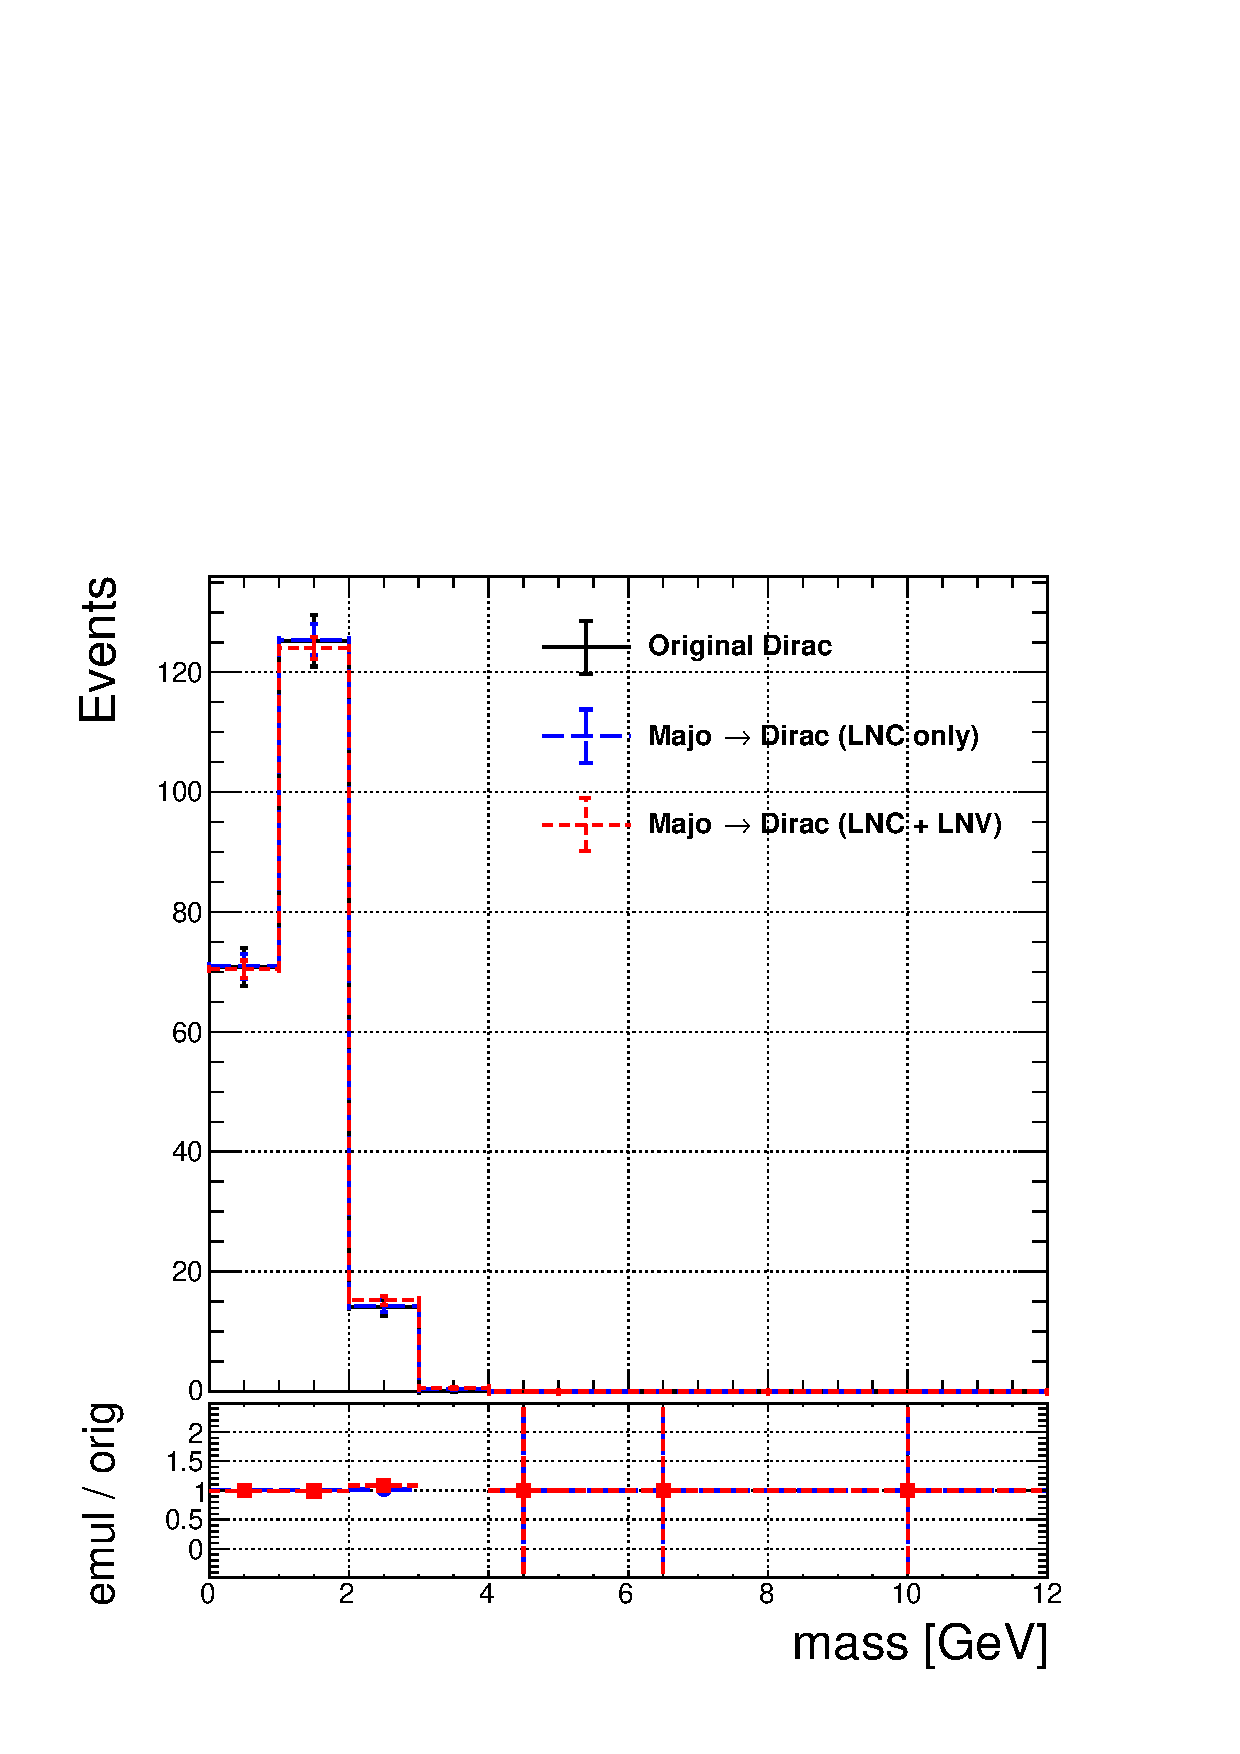
\includegraphics[width = .32\textwidth]{Figures/c4/reweighting/diracReweighting_M-2_V-0p0157162336455_mu_mass_18.pdf}
  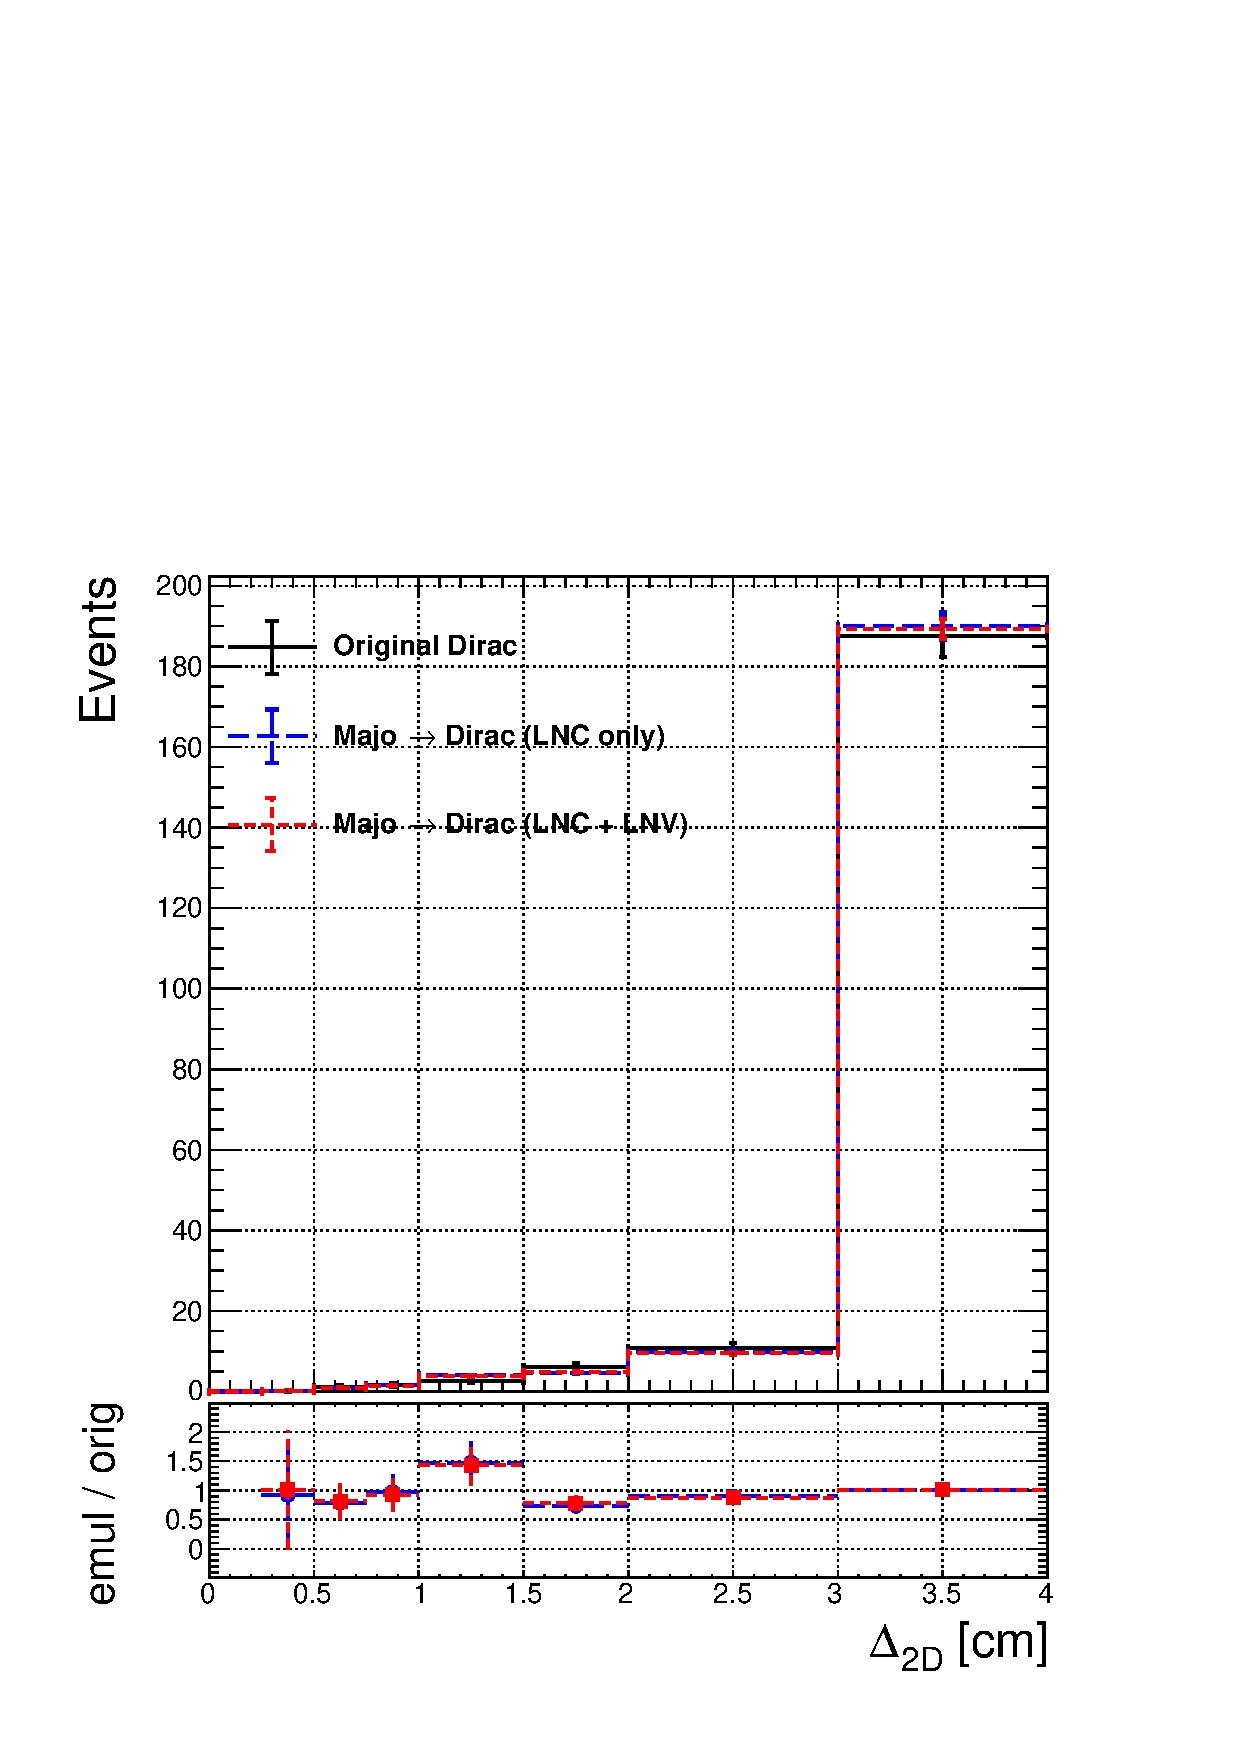
\includegraphics[width = .32\textwidth]{Figures/c4/reweighting/diracReweighting_M-2_V-0p0157162336455_mu_disp_18.pdf}
  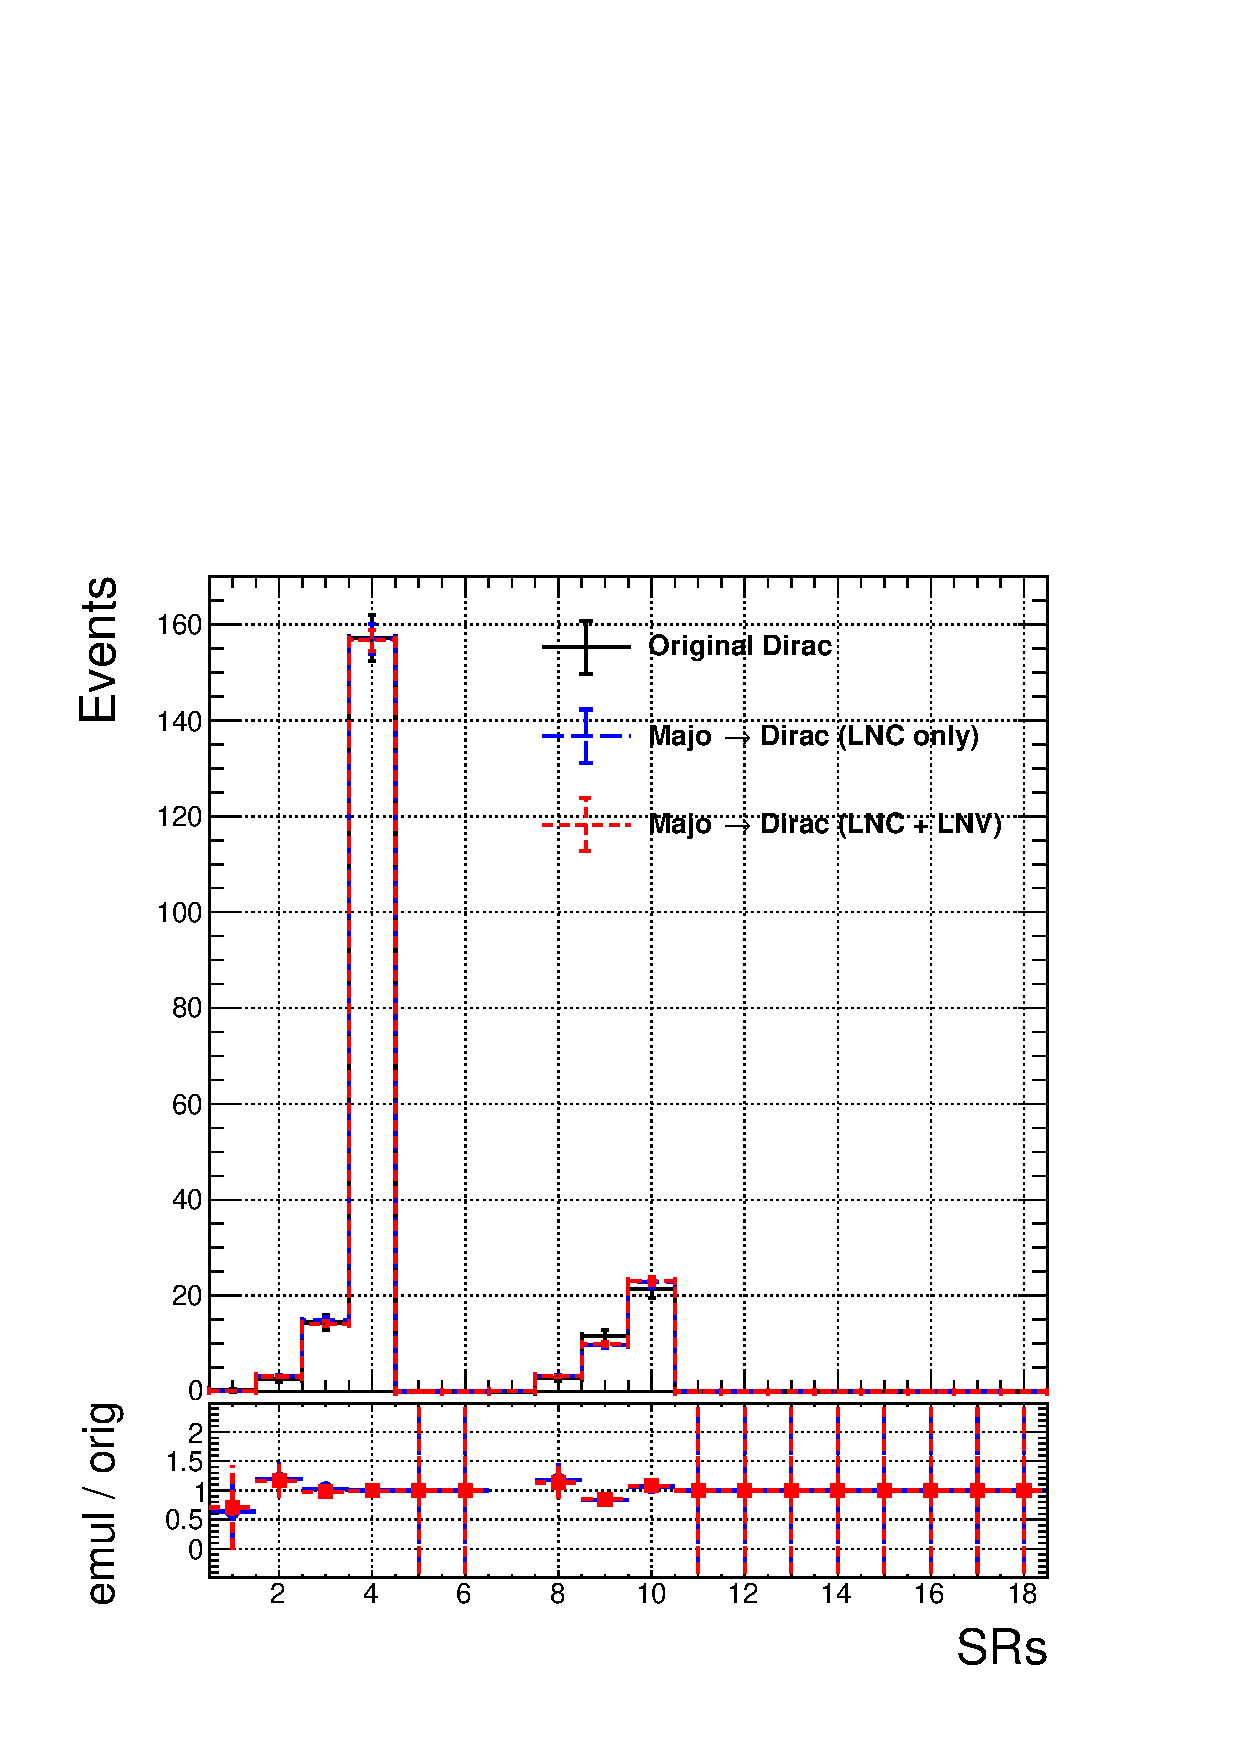
\includegraphics[width = .32\textwidth]{Figures/c4/reweighting/diracReweighting_M-2_V-0p0157162336455_mu_18.pdf}
  \caption{Distributions of the reconstructed dilepton mass \mtwol
    (left), of the transverse displacement of the reconstructed
    HNL decay vertex \Deltwod (middle), and event yields in the
    different analysis categories (right) for a Dirac HNL with
    $\mhnl=2$\GeV and $\mixparm=2.47\times 10^{-4}$ in 2018
    simulation, using three models: a Dirac HNL sample (black), or a
    set of Majorana HNL samples with $\mhnl=2$\GeV and various
    $\mixparm$ values, reweighted to emulate the Dirac scenario with
    $\mixparm=2.47\times 10^{-4}$, using LNC events only (blue) or all
    events (red). \dani} 
  \label{fig:majToDirReweighting}
\end{figure}


\subsubsection{Uncertainty on LL-signal MC cross section}\label{sec:c4lo}
The \texttt{heavyN} model used for generation of Monte Carlo HNL events does not allow for NLO QCD calculations. The simulation of HNL events happens therefore at LO, resulting in large theoretical uncertainties on the cross section (up to $15\%$) that have to cover the effect of the missing higher order QCD corrections and PDF uncertainties.

Instead of relying on these LO uncertainties, a general correction factor for the cross section from LO to NNLO can be derived based on the SM production of \PW\ $\rightarrow$ $\ell$ $\bar{\nu}$ . In HNL production, the only difference from this SM process is the exchange of the SM neutrino by a HNL. The effect of the mass and coupling of the HNL can be factorized in the calculation of the HNL cross section and is not affected by the PDF and scale variations. The dominant effect of these uncertainties appears at the production of the \PW boson, therefore it can be studied in the SM process \PW\ $\rightarrow$ $\ell$ $\bar{\nu}$ , for which recommended values for the cross section at NNLO exist with their corresponding theory uncertainties. Our approach is to get a LO cross section for \PW\ $\rightarrow$ $\ell$ $\bar{\nu}$ calculated with Madgraph using the same exact conditions as the HNL MC production. A correction factor from LO to NNLO can be derived based on this and can then be applied to HNL MC. The PDF and scale uncertainties at NNLO are applied as flat systematic uncertainties to cover the remaining uncertainty on the MC cross section.

It has been checked and verified that the generator conditions are similar between our MC production and the centrally produced W+jets samples, from which the recommended NNLO cross section was taken. The small differences that are present have no significant effect on the cross section calculation. Additionally, lepton universality will allow us to apply the scale factor and uncertainty across all HNL samples, regardless of which lepton flavor(s) they couple with.

The resulting LO cross section for \PW\ $\rightarrow$ $\ell$
$\bar{\nu}$ ($\ell$ = \Pe\ , \PGm\ , \PGt\ ) is 56500 pb. The recommended NNLO value is $61526.7^{+497.1}_{-264.6}\pm 2312.7$ pb where the quoted uncertainties are respectively scale and PDF uncertainties. Assuming uncorrelated uncertainties and taking the maximum of the two asymmetric errors, the combined uncertainty is $61526.7 \pm 2365.5$ pb, an effect of $3.86\%$. This gives a final scale factor of $1.089 \pm 0.042$.

\section{Data sets}\label{sec:c4data}

For each CMS analysis according to the final states we 
select, a specific type of primary datasets (PDs) is used.\\
The definition of the primary datasets (PDs) is intrinsically connected to
the HLT trigger paths (~\ref{sec:triggersystem}). The PD design is centered
around particles reconstructed in the event by the HLT, and follows one simple principle:
grouping together events with similar physics content; for instance, there are
single lepton datasets and double leptons datasets.
Since an event can pass more than one HLT path,
it can enter in more than one primary dataset. At a practical level, possible overlaps among different datasets are
removed by checking run, lumi-section, and event numbers in order to not have twice the same event coming from different PDs.\\


The analysis presented in Chapter~\ref{Chapter5} includes
\texttt{SingleElectron}, \texttt{SingleMuon}, \texttt{DoubleEG},
\texttt{DoubleMuon} and \texttt{MuonEG} primary datasets; the choice was driven by the
multiple trigger requests, both single lepton trigger and
dilepton triggers in order to maximize the trigger efficiency.

The analysis presented in Chapter~\ref{Chapter6} includes only
\texttt{SingleElectron} and \texttt{SingleMuon}; \texttt{DoubleEG} and
\texttt{DoubleMuon} primary datasets are used for background
predictions measurement only. For this specific case the choice was
made considering the limitations due to the presence of displaced
leptons in the final states.
Since (most of) the CMS leptonic triggers are
optimized for prompt lepton identification, it was decided
to use single-electron and single-muon triggers for the
signal selection.\\

The first analysis presented in the following chapters used only 
\Pp collision data collected
by the CMS experiment at center-of-mass energy of 13\TeV
in 2016, corresponding to an integrated luminosity of 35.92\fbinv.\\

The long-lived HNL analysis uses three sets of \Pp collision data
corresponding to three years of data-taking at a
center-of-mass energy of 13\TeV, corresponding to integrated
luminosities of 35.92\fbinv (2016), 41.53\fbinv (2017), and 59.97\fbinv
(2018). 

\section{Summary}\label{sec:summaryC4}
In this chapter an overview of the simulated samples and the data sets
samples is presented.\\
We first introduced the different ``ingredients'' that compose the
background of the analyses presented in Chapters~\ref{Chapter5}
and~\ref{Chapter6}. We tried to explain which SM processes can
contribute and contaminate the signal region falling inside the object and event
selection.  Taking into account the three prompt
leptons final state scenario, we listed the processes that better
mimic the signal signatures while having a sizable branching
ratio and large production cross-sections. 

We described the HNL model adopted in the context of this thesis. The
main features were presented with a large focus on
displaced case. In this framework the re-weighting procedure was
introduced, which is going to be a key point for the 
interpretation of the results in both the prompt and displaced heavy neutral lepton
analyses of Chapters~\ref{Chapter5}
and~\ref{Chapter6}.

Finally details about data taking, data campaigns and primary datasets were presented.


